\documentclass{vgtc}                          % final (conference style)
%\documentclass[review]{vgtc}                 % review
%\documentclass[widereview]{vgtc}             % wide-spaced review
%\documentclass[preprint]{vgtc}               % preprint
%\documentclass[electronic]{vgtc}             % electronic version

\usepackage{mathptmx}
\usepackage{graphicx}
\usepackage{times}
\usepackage{paralist}
\usepackage{subcaption}
\usepackage{listings}
\usepackage{color}

%% Add commands for adding author comments:
\newcommand{\wrs}[1]{\textbf{\textcolor[rgb]{0,0,1}{WRS: #1}}}
\newcommand{\pwo}[1]{\textbf{\textcolor[rgb]{0,1,0}{PWO: #1}}}
%%\newcommand{\bill}[1]{}


%% This turns references into clickable hyperlinks.
\usepackage[bookmarks,backref=true,linkcolor=black]{hyperref} %,colorlinks
\hypersetup{
  pdfauthor = {},
  pdftitle = {},
  pdfsubject = {},
  pdfkeywords = {},
  colorlinks=true,
  linkcolor= black,
  citecolor= black,
  pageanchor=true,
  urlcolor = black,
  plainpages = false,
  linktocpage
}
\usepackage[all]{nowidow}

%% If you are submitting a paper to a conference for review with a double
%% blind reviewing process, please replace the value ``0'' below with your
%% OnlineID. Otherwise, you may safely leave it at ``0''.
\onlineid{308}

%% declare the category of your paper, only shown in review mode
\vgtccategory{Research}

%% allow for this line if you want the electronic option to work properly
\vgtcinsertpkg

%% In preprint mode you may define your own headline.
%\preprinttext{To appear in an IEEE VGTC sponsored conference.}

\title{Cross-platform ubiquitous volume rendering using programmable shaders in
  VTK for scientific and medical visualization}

\author{Aashish Chaudhary\corref{cor1}}
\ead{aashish.chaudhary@kitware.com}

\author{Sankhesh J. Jhaveri\corref{}}
\ead{sankhesh.jhaveri@kitware.com}

\author{Alvaro Sanchez}
\ead{alvaro.sanchez@kitware.com}

\author{Lisa S. Avila}
\ead{lisa.avila@kitware.com}

\author{Kenneth M. Martin}
\ead{ken.martin@kitware.com}

\author{David Lonie}
\ead{david.lonie@kitware.com}

\author{Marcus D. Hanwell}
\ead{marcus.hanwell@kitware.com}

\author{Will Schroeder}
\ead{will.schroeder@kitware.com}

\address{Kitware, Inc., 28 Corporate Drive, Clifton Park, NY 12065, USA}
\cortext[cor1]{Corresponding Author}


\begin{abstract}
\label{abstract}The Visualization Toolkit (VTK) is a popular cross-platform, open source
toolkit for scientific and medical data visualization, processing, and
analysis. It supports a wide variety of data formats, algorithms, and rendering
techniques for both polygonal and volumetric data. In particular VTK's volume
rendering module has long provided a comprehensive set of features such as
plane clipping, color and opacity transfer functions, lighting, and other
controls needed for visualization. However, due to VTK's legacy OpenGL backend
and its reliance on a deprecated API, the system did not take advantage of the
latest improvements in graphics hardware or the flexibility of a programmable
pipeline. Additionally, this dependence on an antiquated pipeline posed
restrictions when running on emerging computing platforms, thereby limited its
overall applicability. In response to these limitations, the VTK community
developed a new and improved volume rendering module, which not only produced
a modern GPU-based implementation, but also augmented its capabilities with new
features such as fast volume clipping, gradient magnitude based opacity
modulation, render to texture, and hardware-based volume picking.
\end{abstract}


\teaser{
  \centering
  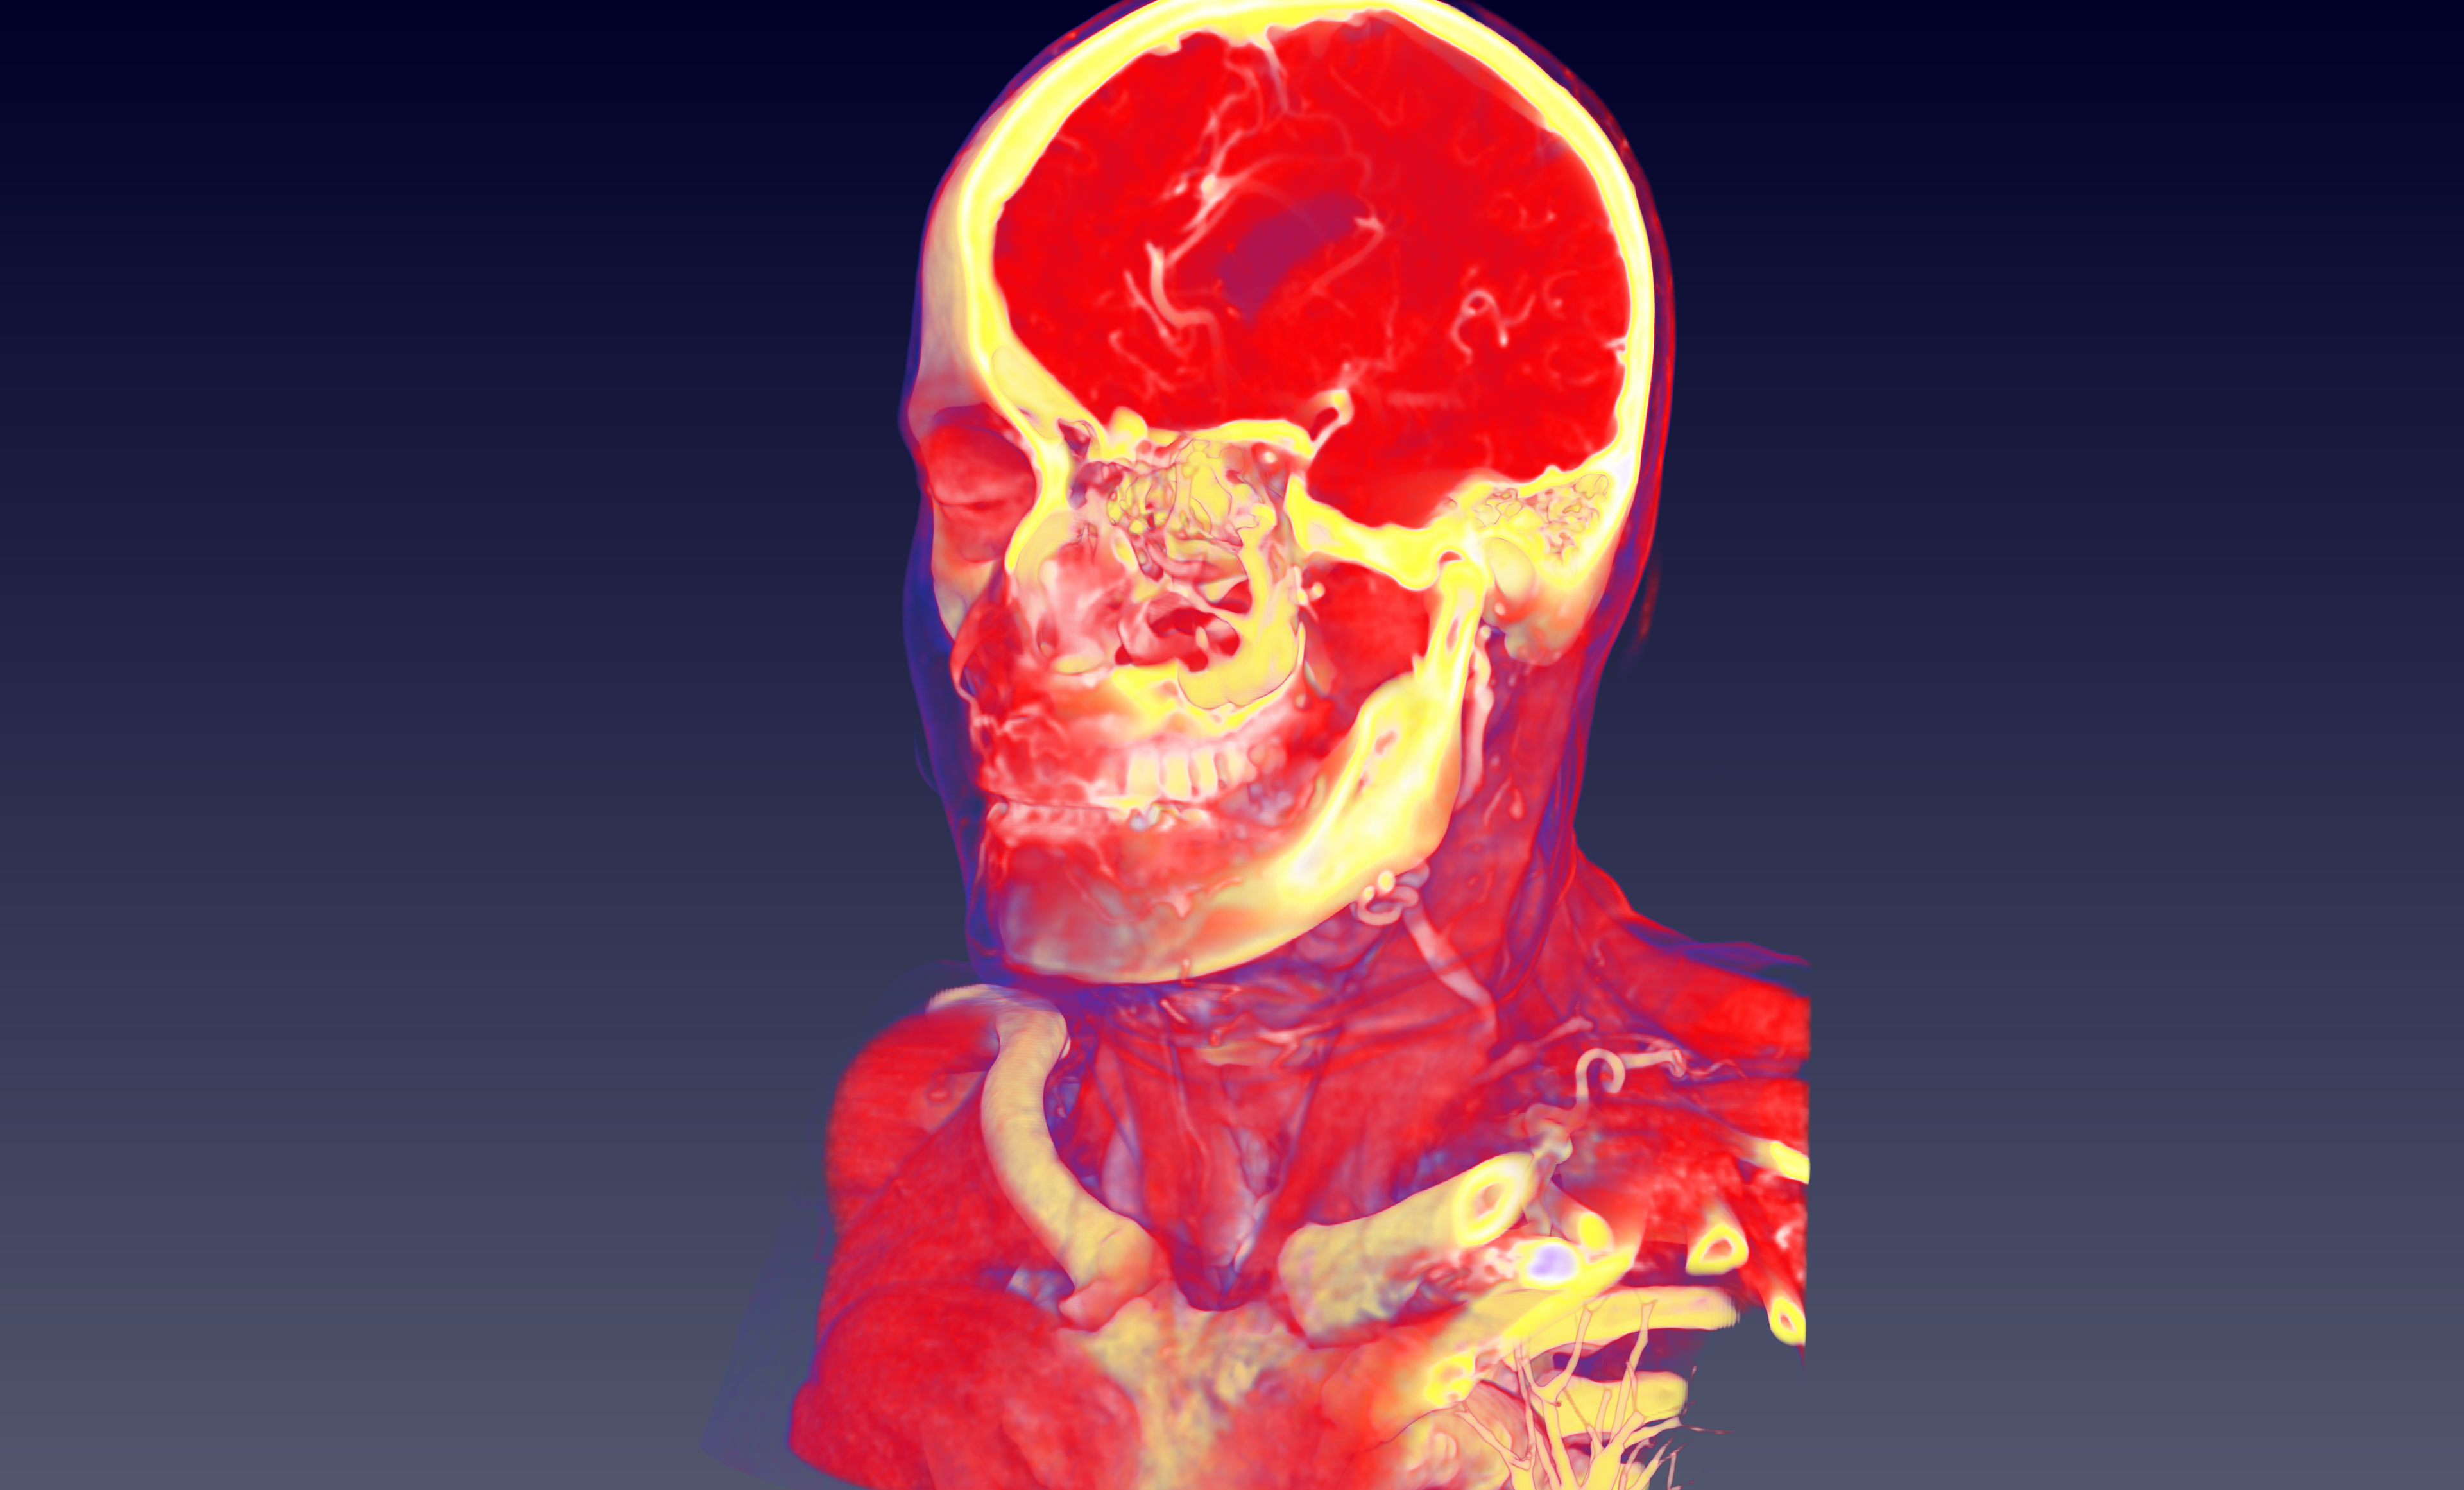
\includegraphics[width=17cm]{HeadClippingOblique.png}
  \caption{A VTK volume rendering example showing oblique clipping plane used for visualization inside human brain.}
  \label{fig:CAVEVolumeViz}
}

\begin{document}

\firstsection{Introduction}

\maketitle

VTK has a long history of volume rendering and, unfortunately, that history is
evident in the large selection of classes available to render volumes. Each of
these methods was state-of-the-art at the time, but given VTK’s 20+ year
history, many of these methods are now quite obsolete. One of the goals of this
work is to reduce the number of volume mappers to ideally just two: one that
supports accelerated rendering on graphics hardware and another that works in
parallel on the CPU. The vtkSmartVolumeMapper would help application developers
by automatically choosing between these techniques based on system performance. 

\begin{figure}[h]
  \centering
  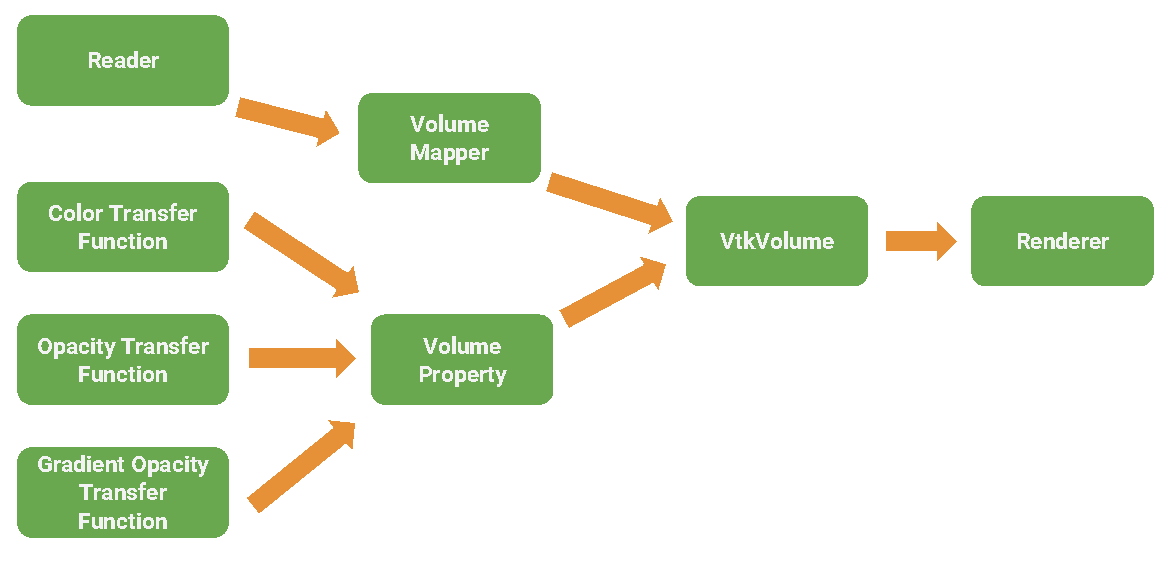
\includegraphics[width=\columnwidth]{vtk_volume_pipeline.pdf}
  \caption{VTK pipeline for volume rendering which is similar to VTK polygonal
    rendering with differences such as transfer functions are defined on the
    property object.}
  \label{fig:pipeline}
\end{figure}%

The main objective of this effort is to create a cross-platform,
multi-functional and high-performance volume renderer that works in both serial
and parallel mode (for example in
ParaView\cite{ahrens_paraview:_2005,ayachit_paraview_2015}). To achieve this,
we have created a replacement for the OpenGL fixed pipeline based
vtkGPUVolumeRayCastMapper. The new mapper, which shares the same name but uses
the OpenGL programmable pipeline, can be used via vtkSmartVolumeMapper or
instantiated directly and replaces the old vtkGPUVolumeRayCastMapper.
Availability of the new mapper with new OpenGL-VTK implementation improved the
management of textures in the mapper and benefited both forms of rendering
(geometry and volume) by sharing common code between them. While volume
ray-casting itself is a well-known technique, developing a volume renderer that
works with variety of data formats and types, supports many essential features
for medical and scientific computing, works on the main commercial platforms
(such as Windows, Mac, and Linux) and performs well at interactive frame rates
with very large datasets is still a challenging task that requires an in-depth
knowledge of the data, graphics pipeline, the VTK framework and the user
requirements.  In the next section, we will cover technical details of our work
that resulted in a sophisticated volume renderer for the VTK community.

% \section{Related Work}
\label{relatedwork}

Volume Visualization enables viewing of three-dimensional data by rendering
sampled function of three spatial dimensions and projecting the translucent
volume onto a 2D projection plane. While many techniques exist for volume
rendering such as marching cubes~\citep{lorensen_marching_1987}, image
splatting~\citep{westover_footprint_1990}, texture
slicing~\citep{rezk-salama_interactive_2000, engel_high-quality_2001} and ray
casting~\citep{hsu_segmented_1993, ma_parallel_1995, ma_scalable_1997,
heng_gpu-based_2005}, ray casting has become one of the most used ones on modern
graphics hardware. Ray casting technique provides a higher quality of rendering
and many ways to optimize the rendering of the volume such as early ray
termination and space leaping~\citep{yagel_accelerating_1993}.

While the Ray Casting a well-known technique and various implementations exists,
the challenge of providing high-quality volume visualization with dataset of
varying size, spacing, and format, with or without the geometry rendering, on
multiple platforms (Desktop, Cave, Head Mounted Displays (HMD)) and Operative
Systems (Apple, Linux, Window) at interactive speed is still a challenge.

Few open-source implementations exist such as
Voreen~\citep{meyer-spradow_voreen:_2009} which initiated at Department of
Computer Science at the University of Münster, Germany in 2004.  It provides
features such as Isosurface Rendering, Maximum Intensity Projection
(MIP)~\citep{wallis_three-dimensional_1989}, support for 1D and 2D transfer
functions, and support for different illumination models (Phong, Tone, Ambient
Occlusion). Both Voreen and VTK uses data-flow networks. However, Voreen is
Volume Visualization library whereas VTK is a Scientific Visualization library
and provides better support for Geometry and Gridded datasets. While Voreen
provides a rapid prototyping environment, VTK volume visualization aims for
production quality, performance, and Ubiquitousness. Additionally, Voreen only
supports high-end desktop devices where as VTK supports multiple platforms
natively enabling researchers bridging the gap between academic research and
open source and industrial contributions.

Another open-source volume rendering ImageVis3D is being developed by the
researchers at the University of Utah~citep{SCI:ImageVis3D}. ImageVis3D is an
application as opposed to a library and provides support for large volume data
visualization, volume visualization on a desktop and mobile device, MIP, 1D and
2D transfer functions amongst many others.  It does not support Virtual Reality
environments and the flexibility of a data-flow networks.  Few other data type
specific volume rendering libraries such as Voxx~\citep{clendenon_voxx:_2002}
and ClearVolume~\cite{royer_clearvolume:_2015} provides visualization of
biological and light-sheet microscopy. PyMOL~\cite{schrodinger_llc_pymol_2015}
provide volume visualization capabilities only to molecular datasets. Finally,
hardware architecture specific volume visualiation libraries such as
OSPRay~\cite{wald_ospray_2017} and NVIDIA\textsuperscript{\textregistered}
Optix\textsuperscript{\texttrademark}~\citep{parker_optix:_2010} provide fast
large volume data visualization capabilities on Intel CPU and Nvidia GPU's but
lack support for non-native hardware.

Other than Voreen and ImageVis3D, many volumes rendering APIs exist, however,
except for Voreen, advanced volume visualization research performed by the
industry and academic communities are not publicly available. By providing an
open source volume rendering engine that supports multiple platforms natively,
researchers can use the engine as a bridge between academic research and open
source and industrial contributions.

\subsection{Approach}
The new vtkGPUVolumeRayCastMapper uses a ray casting technique ~\ref{raycasting} for volume rendering which is a state-of-the-art for volume rendering on modern graphics platforms. Algorithmically, at a high level, it is similar to the older version of this class (although with a fairly different OpenGL implementation since that original class was first written over a decade ago and used GPU assembly code).  One of the main reason we chose to use ray casting due to the flexibility of this technique, which enables us to support all the features of the software ray cast mapper but with the acceleration of the GPU. Ray casting is an image-order rendering technique, with one or more rays cast through the volume per image pixel. VTK is inherently an object-order rendering system, where the GPU renders all graphical primitives (points, lines, triangles, etc.) represented by vtkProp(s) in the scene in one or more passes (with multiple passes needed to support advanced features such as depth peeling for transparency).

The image-order rendering process for vtkVolume is initiated when the front-facing polygons of the volume’s bounding box are rendered with a custom fragment program. This fragment program is used to cast a ray through the volume at each pixel, with the fragment location indicating the starting location for that ray. The volume and all the various rendering parameters are transferred to the GPU through the use of textures (3D for the volume, 1D for the various transfer functions) and uniform variables. Steps are taken along the ray until the ray exits the volume, and the resulting computed color and opacity are blended into the current pixel value. Note that volumes are rendered after all opaque geometry in the scene to allow the ray casting process to terminate at the depth value stored in the depth buffer for that pixel (and, hence, correctly intermix with opaque geometry).

In addition to providing supported features of the old mapper, the new mapper added new capabilities such as clipping on GPU,  gradient opacity, and volume picking amongst many others. In the next few sections, we will cover each of these features in detail.

\subsubsection{Single Pass}
\begin{figure}
\centering

\includegraphics[width=3in]{frontandback.png}
\caption{Front and back faces are rendered for start and end position of the ray.}
\label{fig:raycasting}
\end{figure}


\begin{figure}
\centering
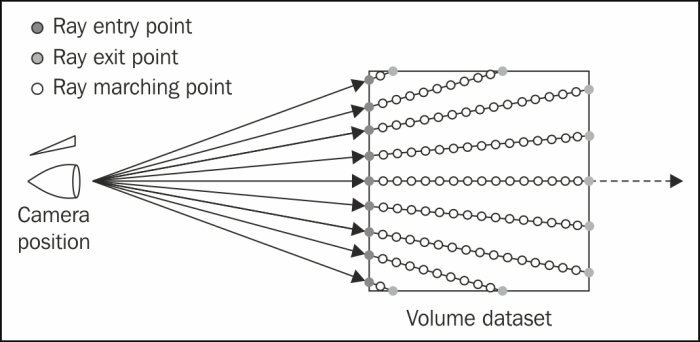
\includegraphics[width=3in]{raycasting.jpg}
\caption{Implementing volume rendering using single-pass GPU ray casting.}
\label{fig:raycasting}
\end{figure}

In a ray-casting algorithm, the entry and the exit point into the volume is needed to determine when to stop the ray-marching. To determine the entry and the exit point, one approach is to render the geometry of the volume bounding box of the volume twice. In the first pass, the front face of the geometry is rendered and in the second pass the backface is rendered as shown in ~\ref{fig:frontandback}. Using the interpolated vertex position and texture lookup, the start and end positions is computed. Instead of this, in vtkGPUVolumeRayCastMapper, entry and exit points are computed based on the fact that the texture extents of the volume is within vec3(1.0), vec3(-1.0) range (and ~\ref{fig:raycasting}). The code below is showing the fragment shader piece that determines whether or not to stop marching the rays depending on the value of stop.
 
 \begin{lstlisting}[breaklines=true]
 bool stop = any(greaterThan(g_dataPos, 
                 ip_texMax)) ||
             any(lessThan(g_dataPos, 
                 ip_texMin));
 \end{lstlisting}
 
 The advantage of such approach is that it requires one less pass and is faster than other approaches since there is no texture generation or lookup happens for determining the termination of the ray.
 
 
\subsubsection{Dynamic Shader Generation}
In the new \texttt{vtkOpenGLGPUVolumeRayCastMapper} all the operations are performed on the GPU. The advantage of this approach was a more streamlined code that is easier to maintain and debug. This approach also provided an opportunity to rework how to support different features without having too many branches in the shader code or having to send all the options to the shader because that would have been detrimental to the performance. In the new \texttt{vtkOpenGLGPUVolumeRayCastMapper}, the shader is dynamically composed by the mapper. For this to work, we have introduced tags in a vertex, or fragment shader which are then replaced by the \texttt{vtkShaderComposer} depending on the option enabled or chosen by the application code. For instance, the skeleton fragment shader defines tags as shown below:
 
 \begin{lstlisting}
//VTK::Base::Dec

//VTK::Termination::Dec 
\end{lstlisting}

At the run time then \texttt{//VTK::Base::Dec} is then replaced by the code shown below. 

To define a structure, we have chosen a strategy that separates the tags in found category: 

1. Declaration (::Dec)
The tags belong to this group are meant to declare variables or function outside the main execution of the shader code. The variables defined are uniform, varying, and user-defined global variables. The functions defined are typically perform operations that are repetitive in nature such as computing color of a fragment. 

2. Initialization (::Init)
The tags belong to this group are meant to initialize variables inside the main execution function of the shader but before the ray-casting loop in the fragment shader. An example of such code includes computation of the initial position of ray and direction of ray traversal.

3. Implementation (::Impl)
The tags belong to this group are the variables or functions or the combination of both that perform the actual operation of clipping, cropping, shading, etc. on one, two, or four component volume data. The implementation code used local and global variables and optimized for performance reasons as they are executed as long as the ray is traversing inside the volume and didn't run into a termination condition which is checked every time.  

4. Exit (::Exit)
The tags belong to this group perform final computation such as the final color of the fragment. These tags are placed outside the ray-casting loop and typically contain numeric assignments.

\subsubsection{Lighting / Shading }
The old mapper supported only one light (due to limitations in OpenGL at the time the class was written). The \texttt{vtkFixedPointRayCastMapper} supports multiple lights, but only with an approximate lighting model, since gradients are precomputed and quantized, and shading is performed for each potential gradient direction regardless of fragment location. The new mapper accurately implemented the VTK lighting model to produce high quality images for publication. To support this, depending on the light type (point, directional, and positional), the lighting parameters are sent to the shader which then performs the per pixel lighting calculations. The number of lights is limited to six mostly because of the performance reasons as the interactive performance goes down significantly with each light added to the scene. The Phong shading lighting model is used for volume rendering lighting. Phong lighting requires normals which have to be computed for each fragment. The normal calculation is done by first computing the gradient and then scaling the gradient by the spacing between the cells. The gradient is computed by reading the scalar values form the neighboring cdells using the offset vector that stores the step size based on the bounds of the volume. 

\subsubsection{Volume Picking}
Picking in the context of volume rendering is the determination of which voxel user has clicked using a pointing device such as the mouse. Picking is one of most basic operations users performs to interact with a 3D scene. VTK legacy volume mappers support picking through an instance external to the mapper itself called ~\texttt{vtkVolumePicker}.  This class casts a ray into the volume and returns the point where the ray intersects an isosurface of a user specified opacity. This technique has certain limitations given that the picking class does not have enough information to correctly account for clipping, transfer functions and other parameters which define how the mapper renders internally, this reduces its reliability on the actual objects being picked. The inherent flexibility of the glsl-based implementation of the new mapper enables seamless integration with the ~\texttt{vtkHardwareSelector}'s interface, which allows a consistent selection of objects in a scene regardless of whether it is geometric or volumetric data.  Providing picking support directly within the fragment shader of the volume mapper ensures high selection accuracy even in situations where a volume intermixes with geometry in seemingly cumbersome ways or advanced features like when clipping planes are enabled (what you see is what you pick). Given the readily available picking styles supported by ~\texttt{vtkHardwareSelector} (e.g. ~\texttt{vtkAreaPicker}), it is possible to make a selection of a specific set of voxels.

\subsubsection{Volume Texture Streaming}
An intrinsic limitation of volume rendering is that the 3D volume data to be rendered does not always fit into the graphics memory of a system. Such limitation becomes increasingly important to address now that the new mapper provides support for mobile architectures.
A relatively simple method when dealing with a large volume is the volume streaming approach also commonly known as bricking in which the volume is split into several blocks so that a single sub-block (brick) fits completely into GPU memory.  Each sub-block is stored in main memory and streamed into GPU memory for a rendering pass one at a time (in a back-to-front manner for correct composition). The sub-blocks are rendered using the standard shader programs and alpha-blended with each other by OpenGL. Streaming the volume as separate texture bricks certainly, imposes a performance trade-off but acts as a graphics memory expansion scheme for devices that would not be able to render a higher quality volume otherwise.

\subsubsection{Dual Depth Peeling}
 
 
\subsubsection{Render to texture}
Typically the mapper uses a single pass rendering approach in which the 3D volume data is rendered on screen, the default framebuffer that contains a color a and a depth buffer. In games and other graphics applications render to texture approach is used to support advanced visual rendering technique such as deferred shading. Render to texture technique uses rendered output from one pass to modify/enhance the output of another rendering passes. Unlike to this, the volume mapper enables rendering to an OpenGL FrameBufferObject (FBO) and obtaining the pixel data from the FBO via simple image retrieval calls. The mapper supports an application to grab color and depth information as texture or VTK image data. The color data is simply the pixel representation of the rendered volume whereas depth data consists of a grayscale image depicting how deep each voxel is in the scene. When an application enables render to texture mode, a framebuffer object is created and used, the vertex and fragment shader are generated, color and depth buffers are cleared, and the color is set to white with a value of zero alpha. The value of zero alpha is used so that applications can safely ignore the transparent pixels and the color buffer is set to white color because white represents the maximum depth, that is the depth of the far plane. In the render to texture pass, the fragment shader writes to color and depth target and to write the depth information it uses the depth of first non-transparent voxel.

\subsubsection{Mobile Support}
The decision to use OpenGL 3 or higher enabled volume rendering to support mobile devices (iOS and Android devices) as OpenGL ES 3.0 supports 3D textures. However the OpenGL ES does not support all of the texture format types, and therefore, new texture formats are added with compile time switch to enable or disable them depending on whether the platform is desktop or mobile. One such example is capturing of depth buffer since that is not yet supported on the mobile platform.  Since typically interactions on mobile devices require touch interactions, the new rendering system added support for multiple touch events such as using two fingers to translate, rotate, and zoom the camera. With minor feature-set exceptions, the new volume mapper works on mobile devices enabling developers to build sophisticated applications for the scientific community.

\subsubsection{Optimizations and Edge-Cases}
The new \texttt{vtkOpenGLGPUVolumeRayCastMapper} is more than just a ray cast mapper implementation. It is designed to work on multiple platforms and developed to perform volume rendering at interactive frame rates. To achieve interactive frame rates and to handle edge cases, we have implemented following optimizations in the new mapper. 

\begin{itemize}
\item Clipping plane optimization 
In VTK a user can place multiple planes at desired angles to clip the volume. This technique is essential for many medical use-cases. Since only one side of clip planes needs to be traversed, performing any sort of ray cast on the clipped side is wasteful. Hence a simple optimization is to move the starting point of the ray on the plane by projecting the ray onto the plane in the view direction. 

\item Eye Too Close to the Volume
When the eye is too close to the volume, the near plane could clip the volume visible bounds resulting in OpenGL clipping removing the geometry from rendering. In such cases the bounding box of the volume that defines the texture coordinates and hence define a surface to start casting the ray needs to be clipped. To handle such scenario, a plant-box interaction is added. So far evey move of the camera is funding invokved checking if the geomtry of the volume needs to be clipped.

\item Support for Double and Long Long Data Type


\end{itemize}
\subsection{Results}
By using the approach described in the previous section, the new mapper grew capable of providing critical features for medical and scientific computing. This section describes each of these features in sufficient detail in the following text.

\newcommand{\ignore}[1]{}

\subsubsection{Stochastic Jittering}
Because ray-casting effectively samples a discrete signal (voxel values along the ray trajectory), the distance between those sampling points heavily influences how accurately the volume data is represented.  Due to well established limitations described by the sampling theorem, low sampling rates may result in aliasing effects 
often referred to as wood-grain artifacts in the context of volume rendering \ignore{\cite{RTVG_jittering}}. Reducing the distance between samples neutralizes these artifacts but takes an important toll on performance.


The mapper supports stochastic jittering, which is an alternative technique to counteract wood-grain artifacts by adding a random offset to the rays in the viewing direction thereby breaking the coherence between neighboring fragments which causes the aliased patterns become apparent (Figure~\ref{fig:jittering}).  Jittering is implemented by creating a random noise texture (using \texttt{vtkPerlinNoise}) and applying the offset to the ray's starting point, thus has a much lower performance penalty than reducing the sampling distance.

%\begin{figure}
%\centering
%\includegraphics[width=2.5in]{Jittering.png}
%\caption{Figure . Left: A sample rendering exhibiting wood-grain artifacts. Right: The same rendering with stochastic jittering on.}
%\label{fig:jittering}
%\end{figure}

\subsubsection{Clipping}
A set of infinite planes can be defined to clip the volume to reveal inner detail, as shown in Figure 4.  Clipping is implemented by determining the visibility of each sample along the ray according to whether that location is excluded by the clipping planes.A set of infinite clipping planes can be defined to clip the volume to reveal inner detail, as shown in Figure 4.  Clipping is implemented by determining the visibility of each sample along the ray according to whether that location is excluded by the clipping planes.

\subsubsection{Cropping}
Cropping refers to 27 regions that defined by two planes along each coordinate axis of the volume and can be independently turned on (visible) or off (invisible) to produce a variety of different cropping effects, as shown in Figure~\ref{fig:cropping}. Cropping is implemented by determining the cropping region of each sample location along the ray and including only those samples that fall within a visible region.

\begin{figure}
\centering
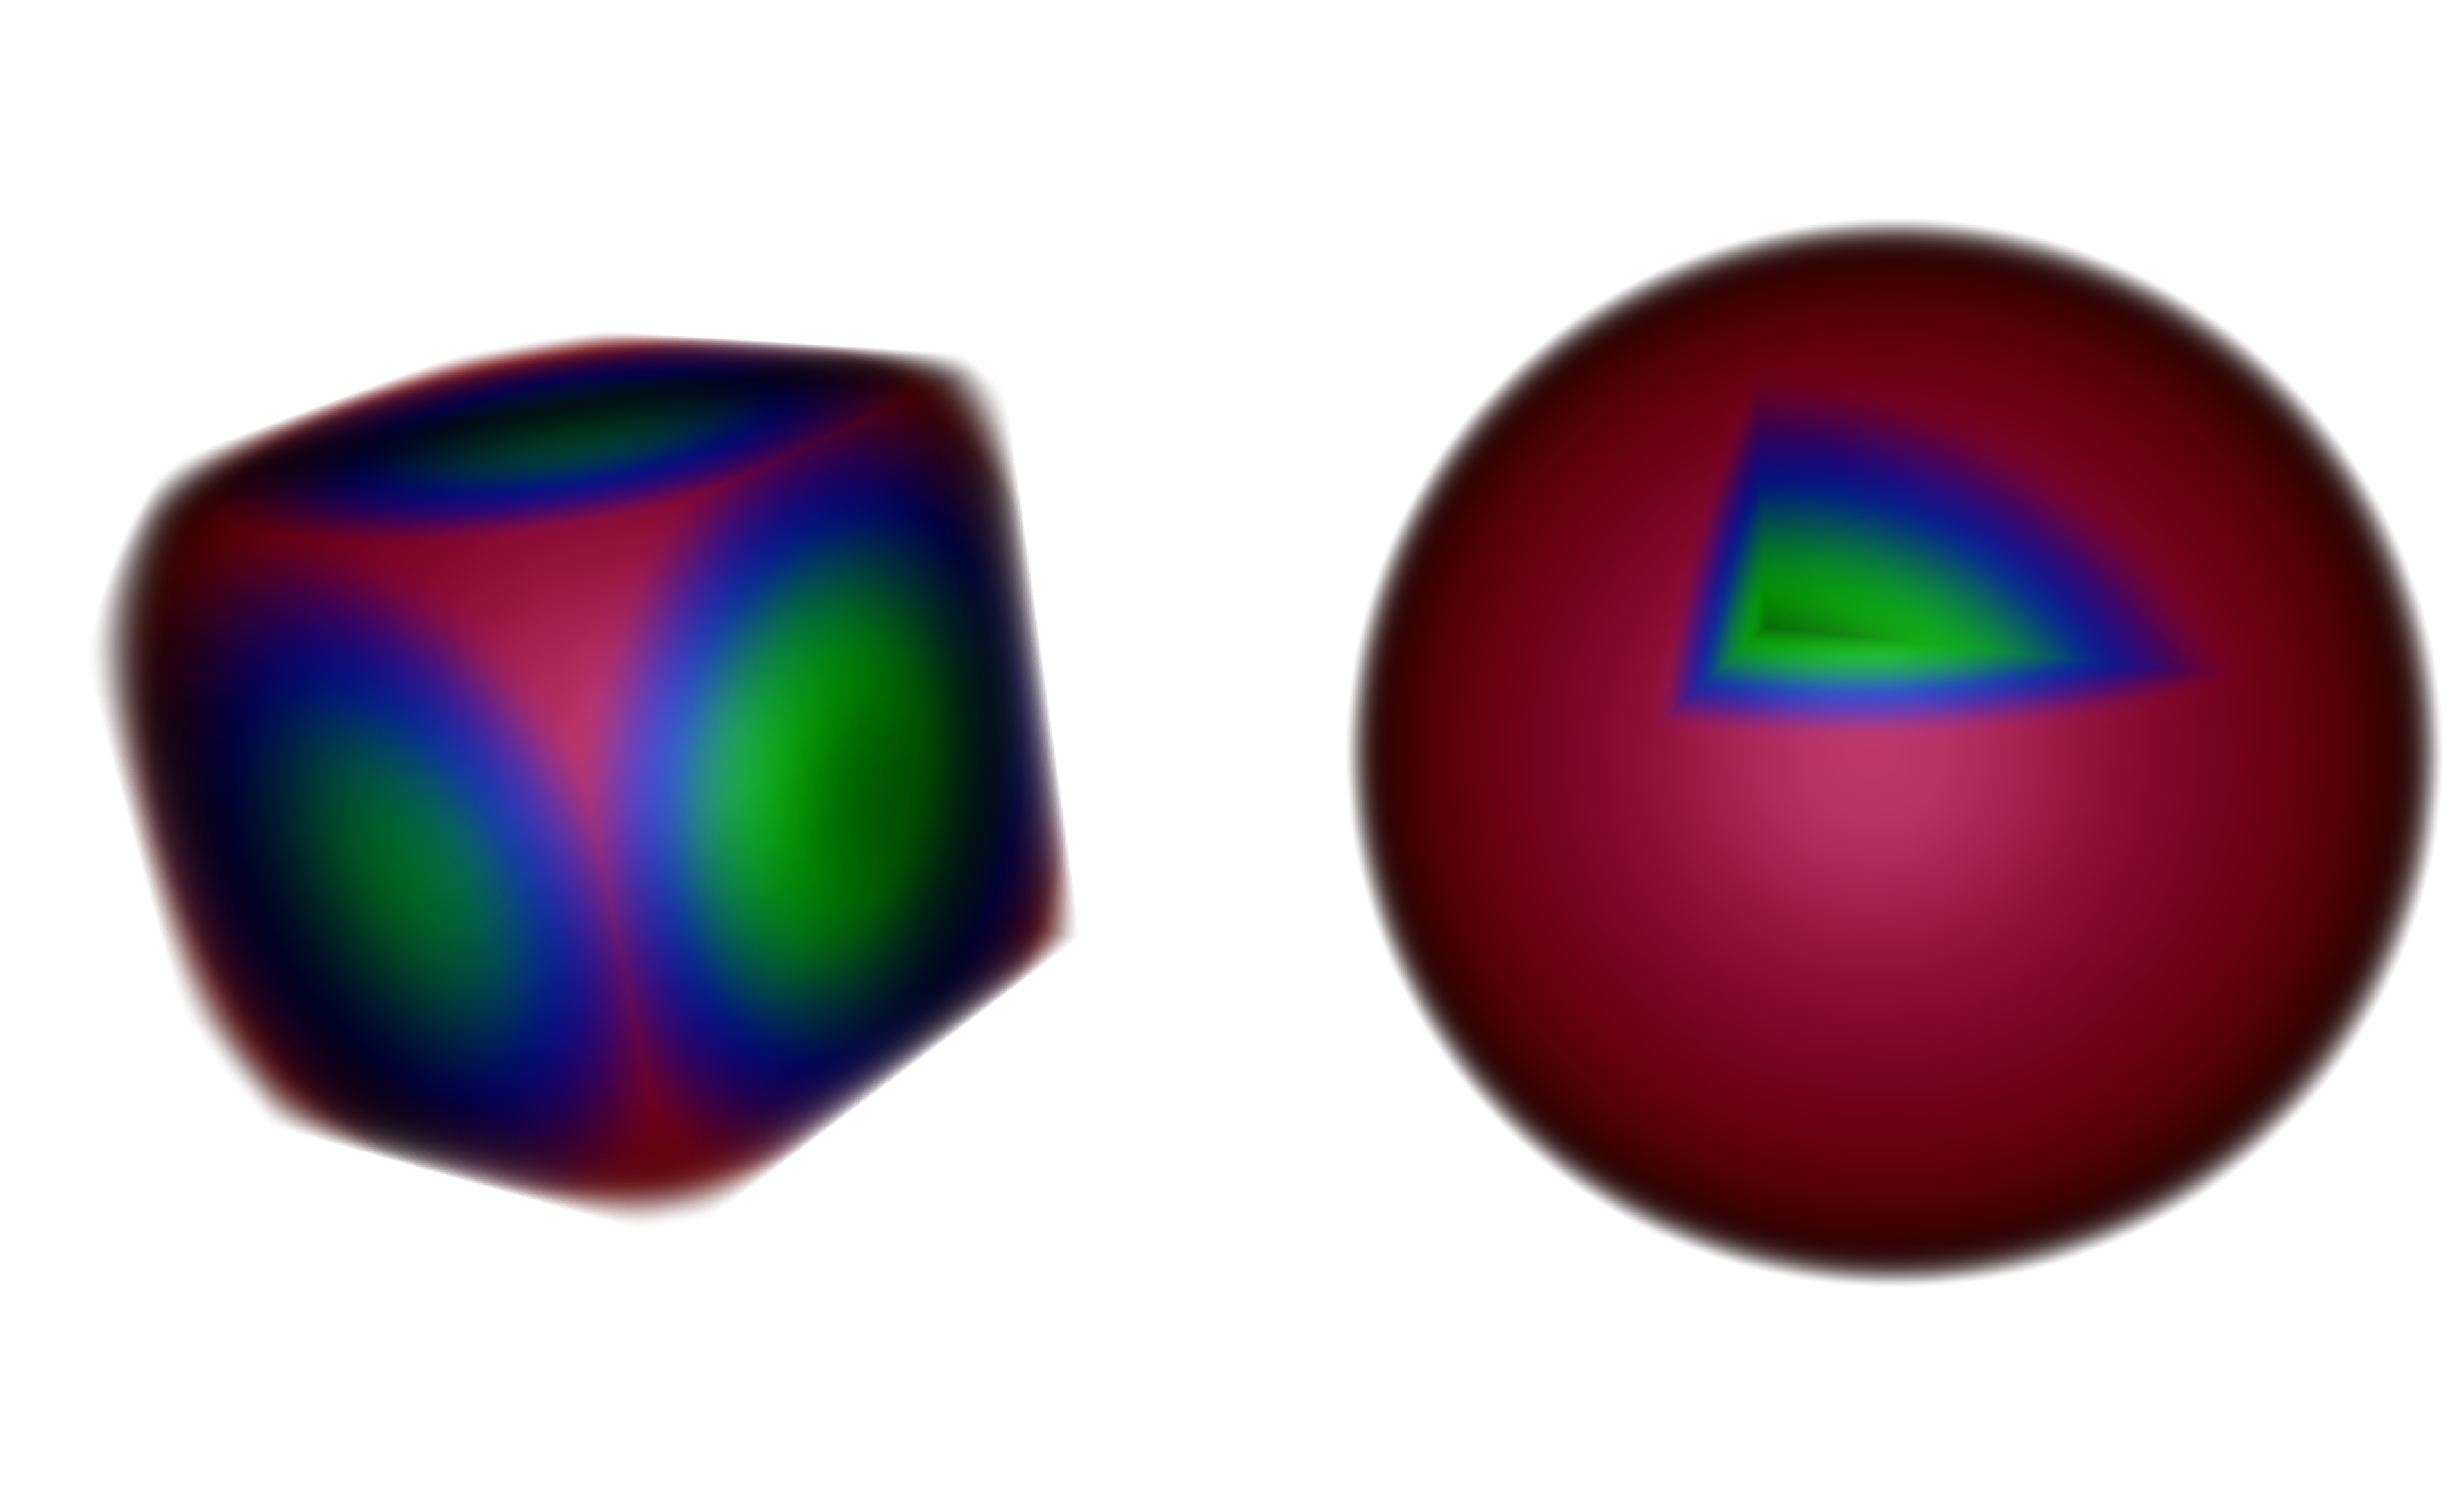
\includegraphics[width=2.5in]{SphereCropping.png}
\caption{Figure 3. A sphere is cropped using two different configurations of cropping regions.}
\label{fig:cropping}
\end{figure}

\subsubsection{Wide Support of Data Types} 
The vtkGPURayCastMapper supports most data types such as short, int, float, and double and both point and cell data types. Bias are scale are computed and applied to the scalars in the fragment shader to normalize the scalars between 0-1 range. 

\begin{figure}
\centering
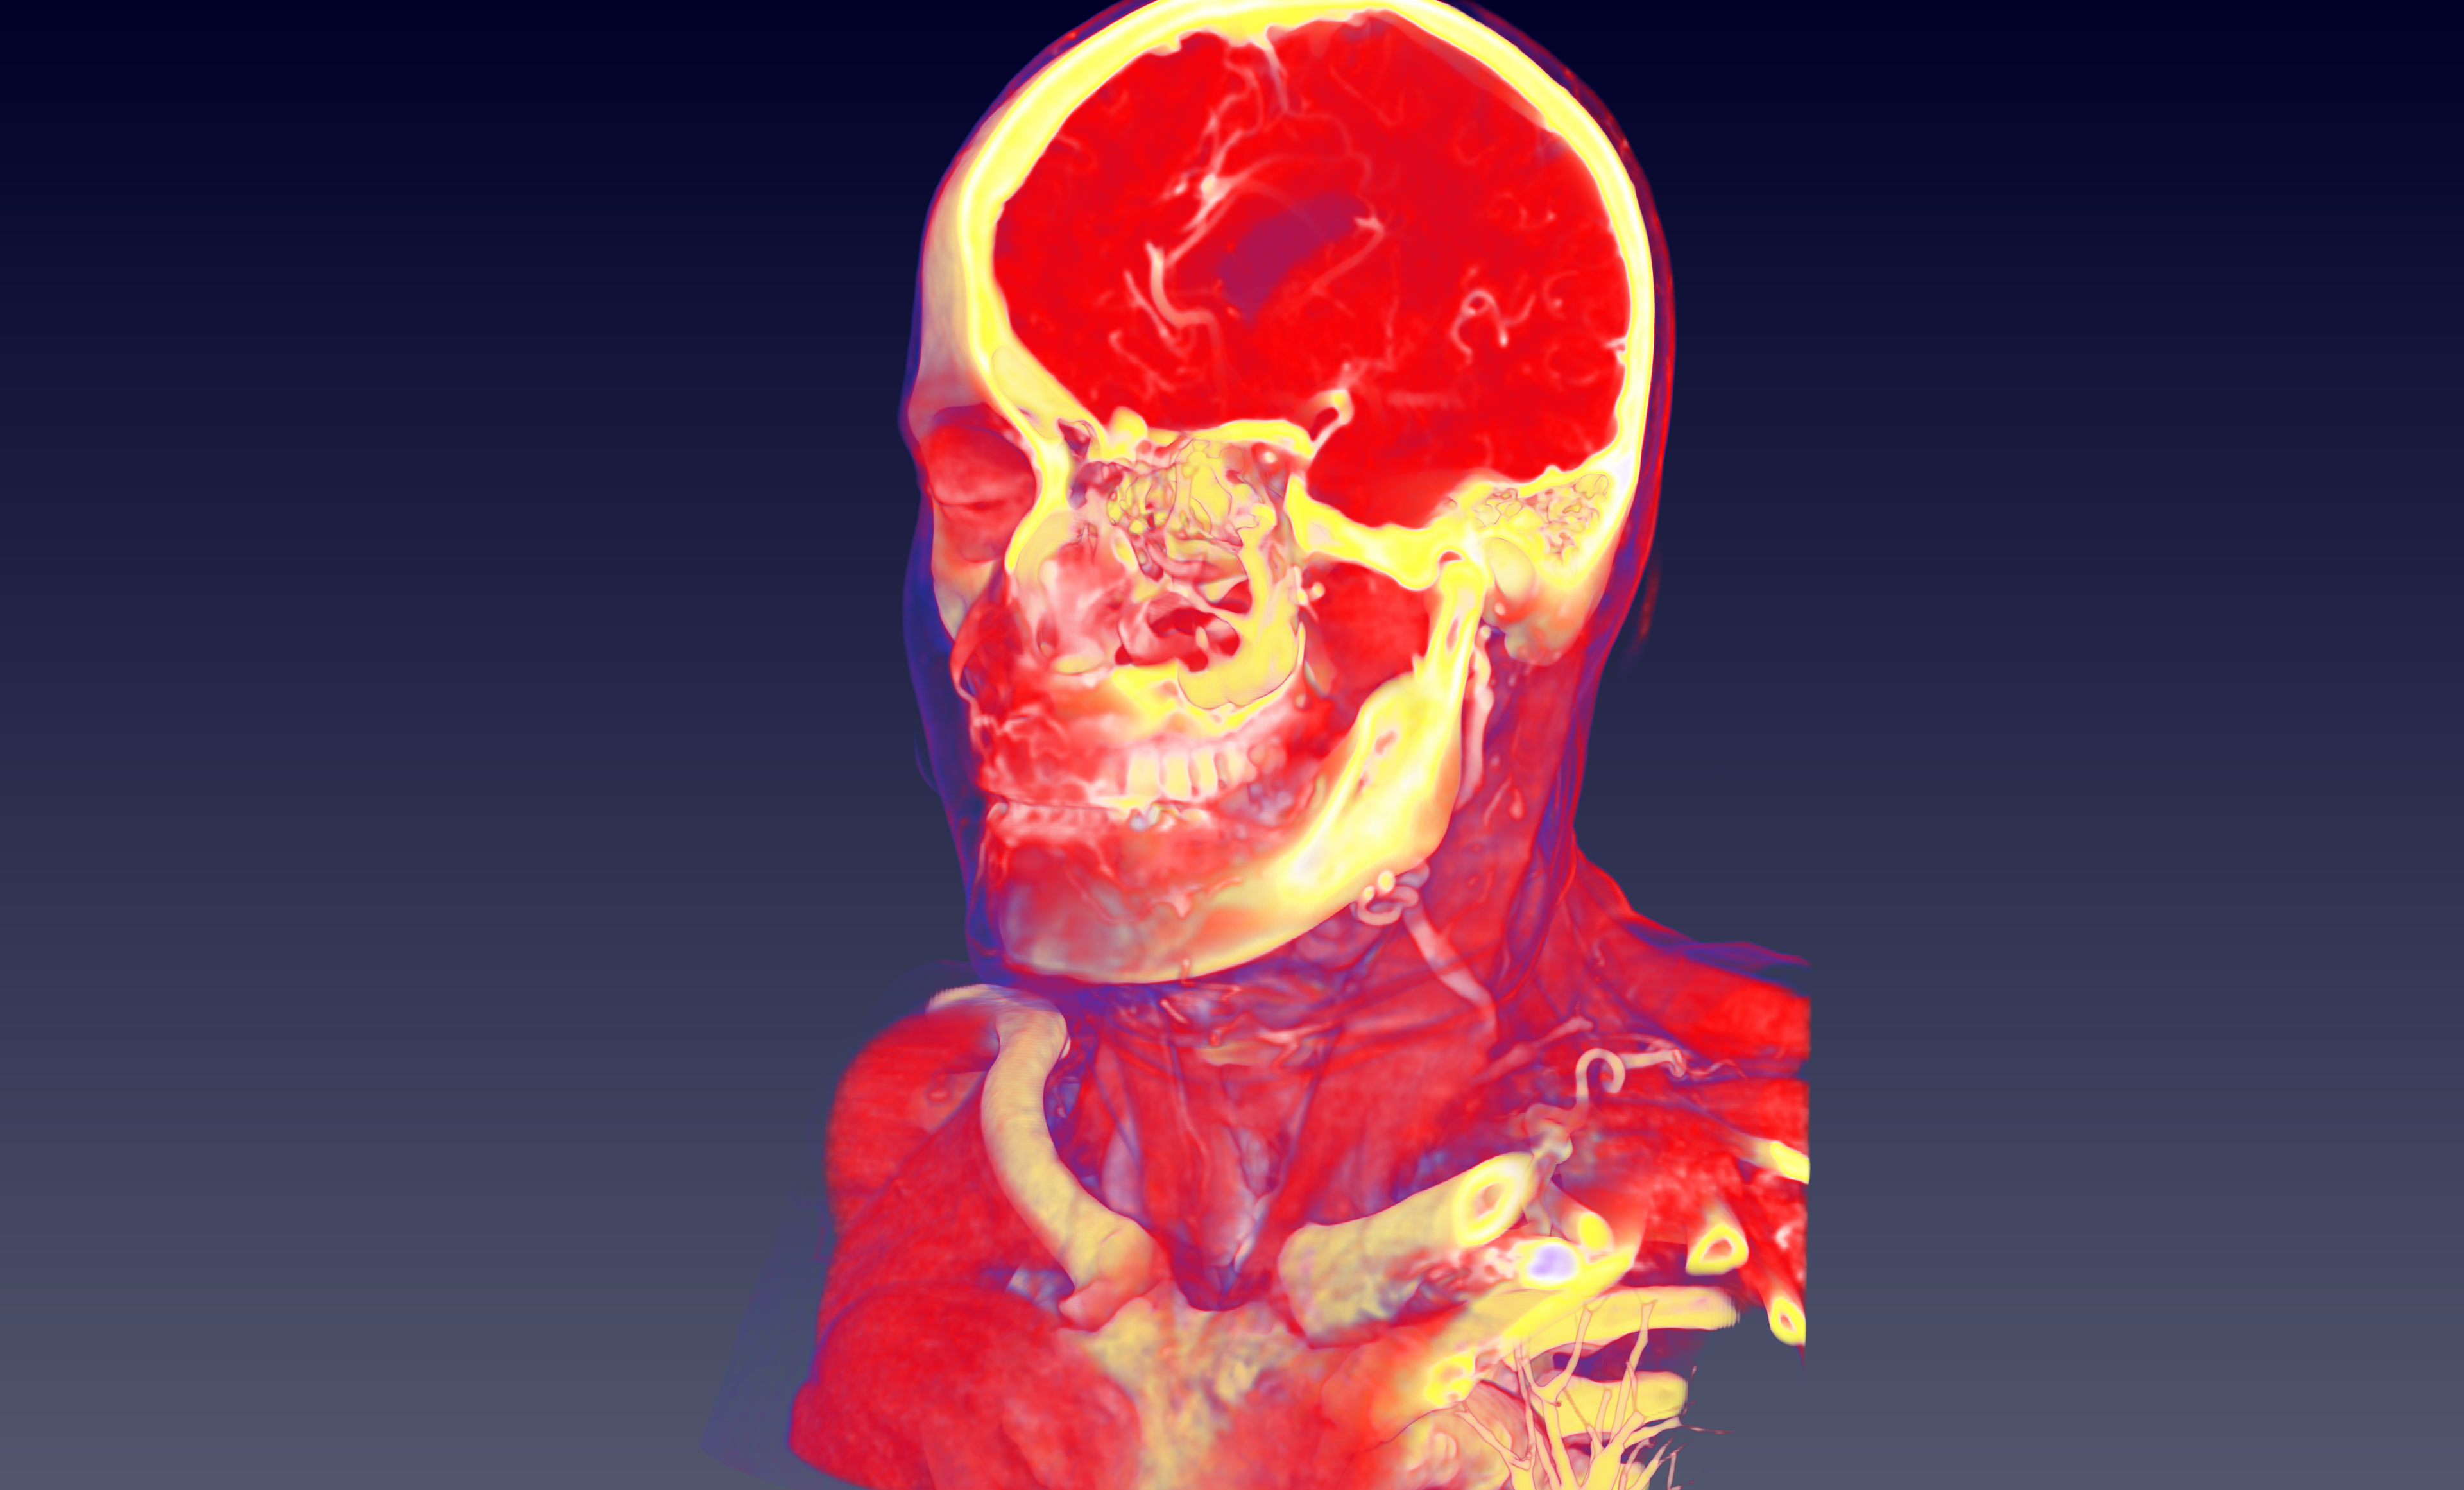
\includegraphics[width=2.5in]{HeadClippingOblique.png}
\caption{Figure 4. Top: An example of an oblique clipping plane. Bottom: A pair of parallel clipping planes clip the volume, rendered without (left) and with (right) shading.}
\label{fig:clipping}
\end{figure}

\subsubsection{Blending Modes *Sankhesh to add new blending mode}
The mapper supports composite blending, minimum intensity projection, maximum intensity projection, and additive blending. Each of these blending modes are useful for a particular use-case in medical computing. The most common one which is also the default is the composite blending mode. See Figure~\ref{fig:blendingmodes} for an example of composite blending, maximum intensity projection, and additive blending on the same data.

\begin{figure*}
\centering
\begin{subfigure}{.6\columnwidth}
    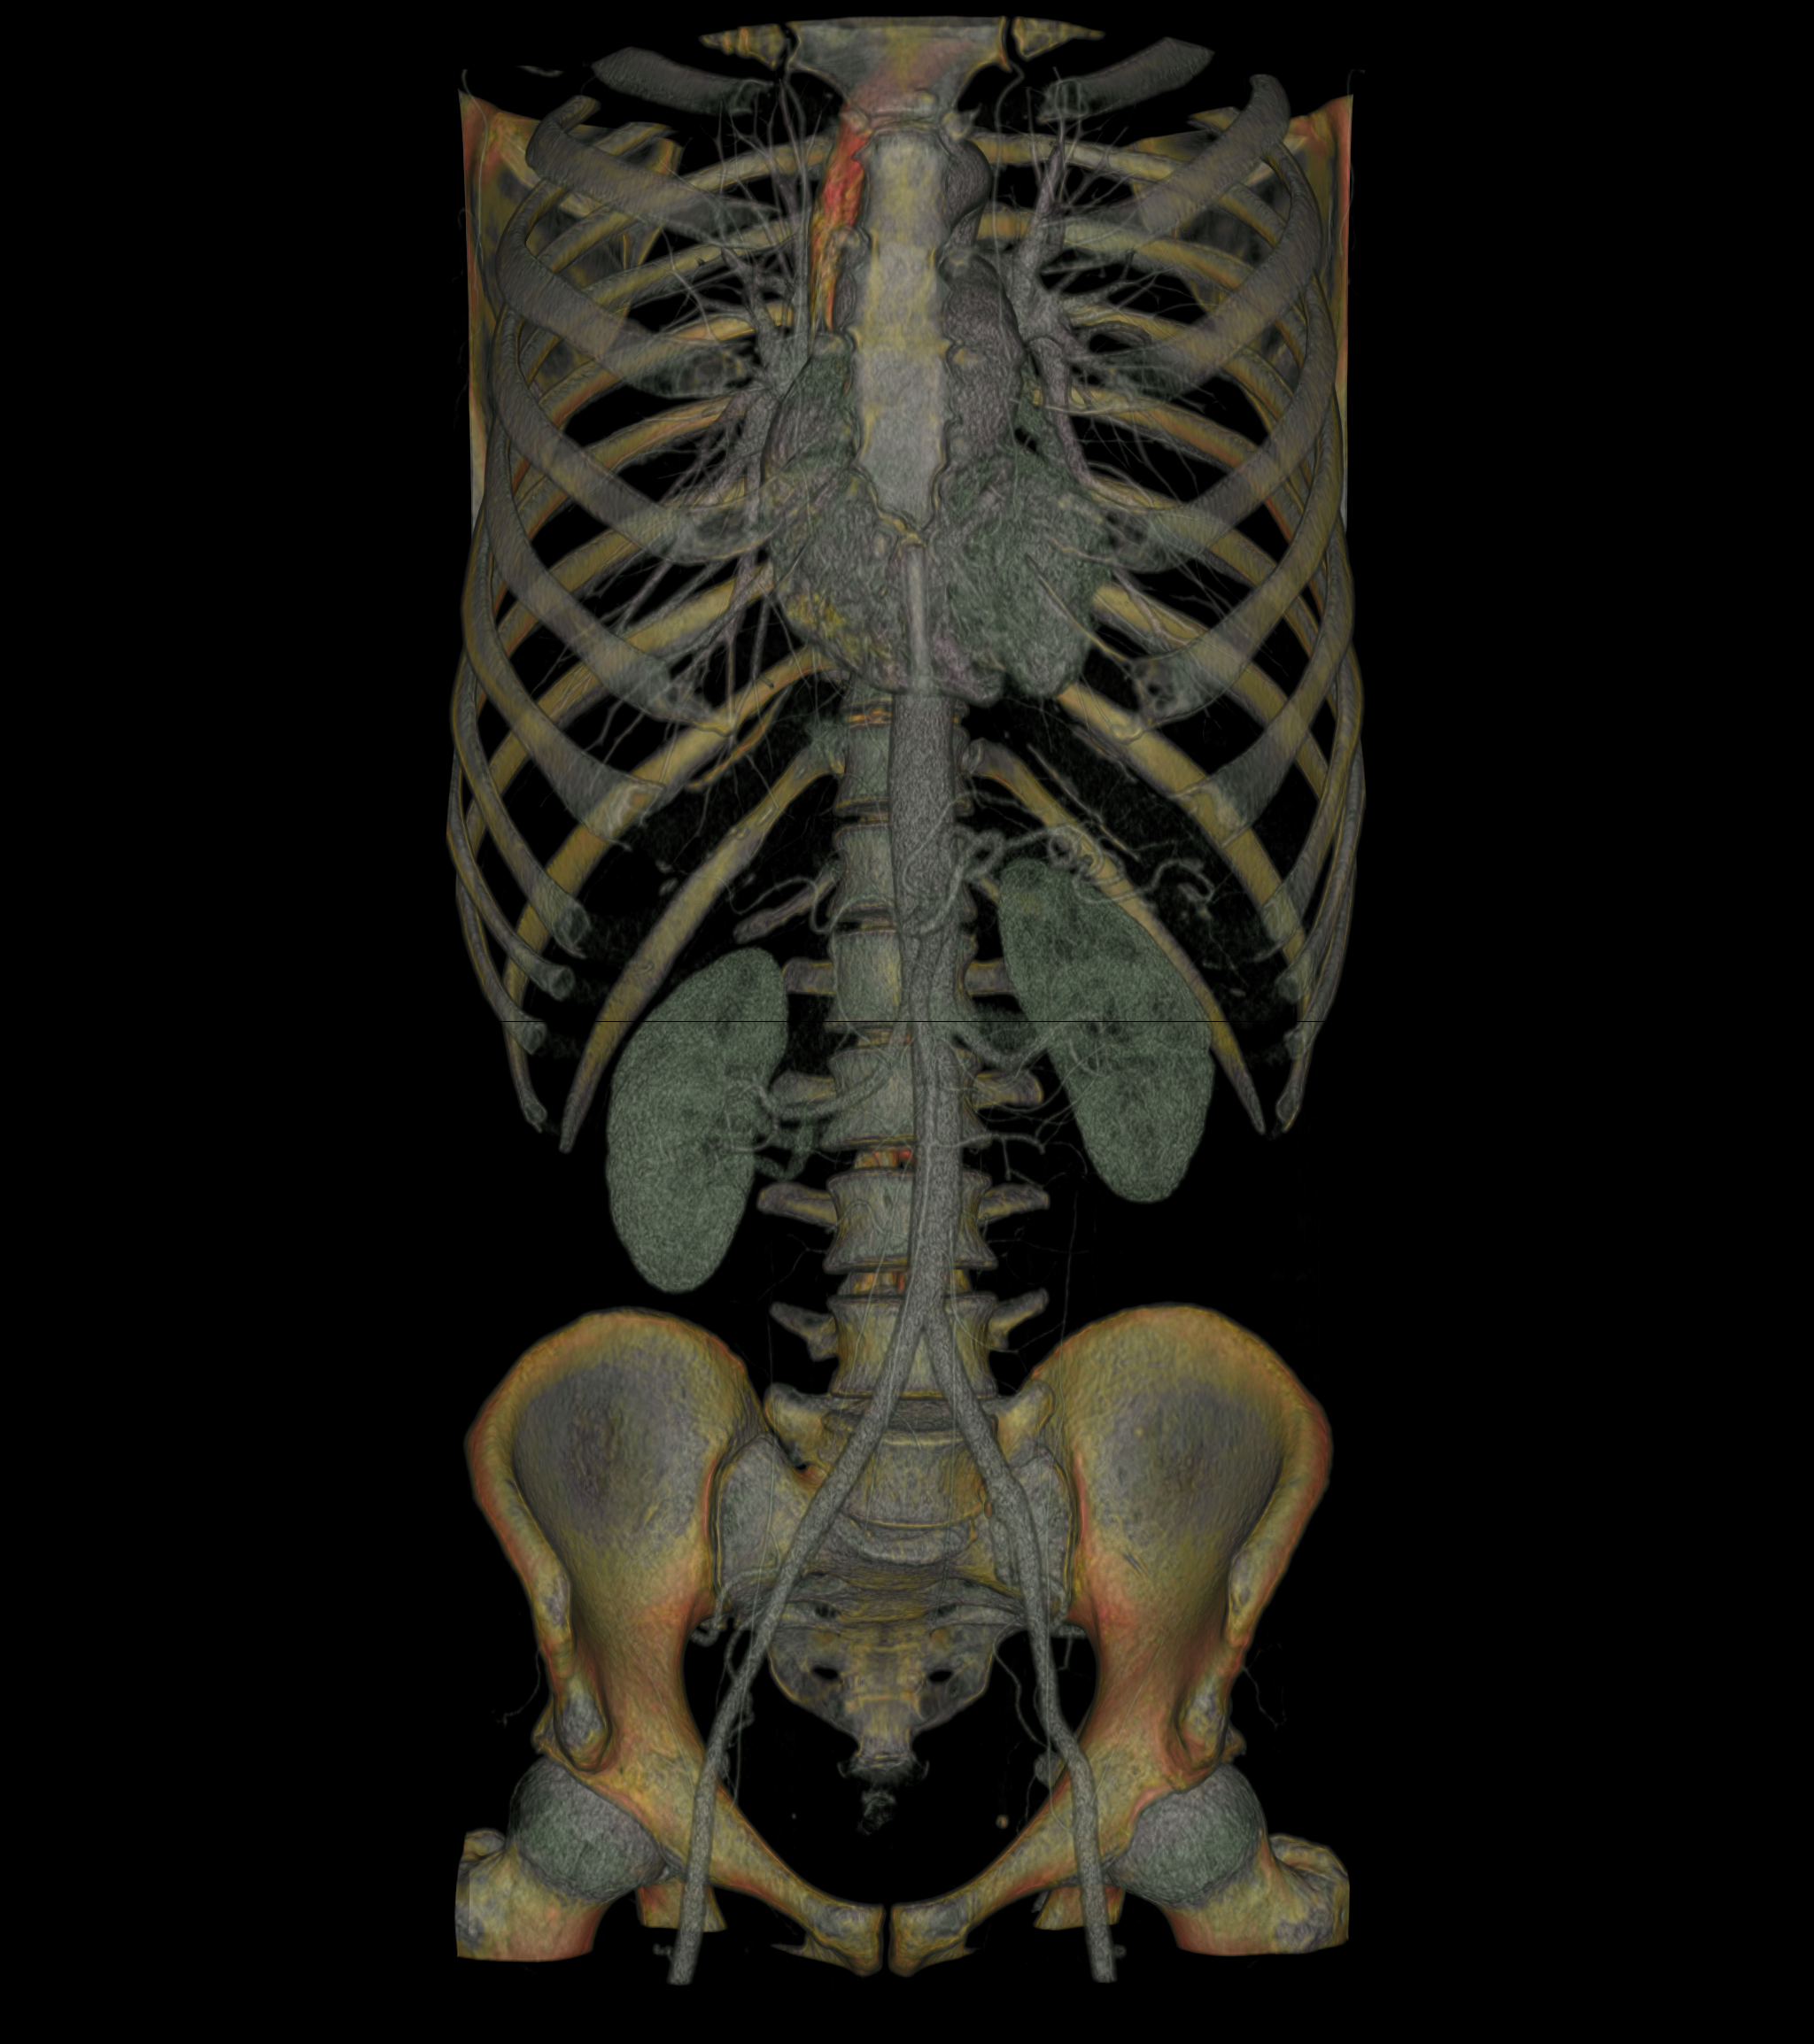
\includegraphics[width=\columnwidth]{TorsoBlendingComposite.png}
\end{subfigure}
\begin{subfigure}{.6\columnwidth}   
    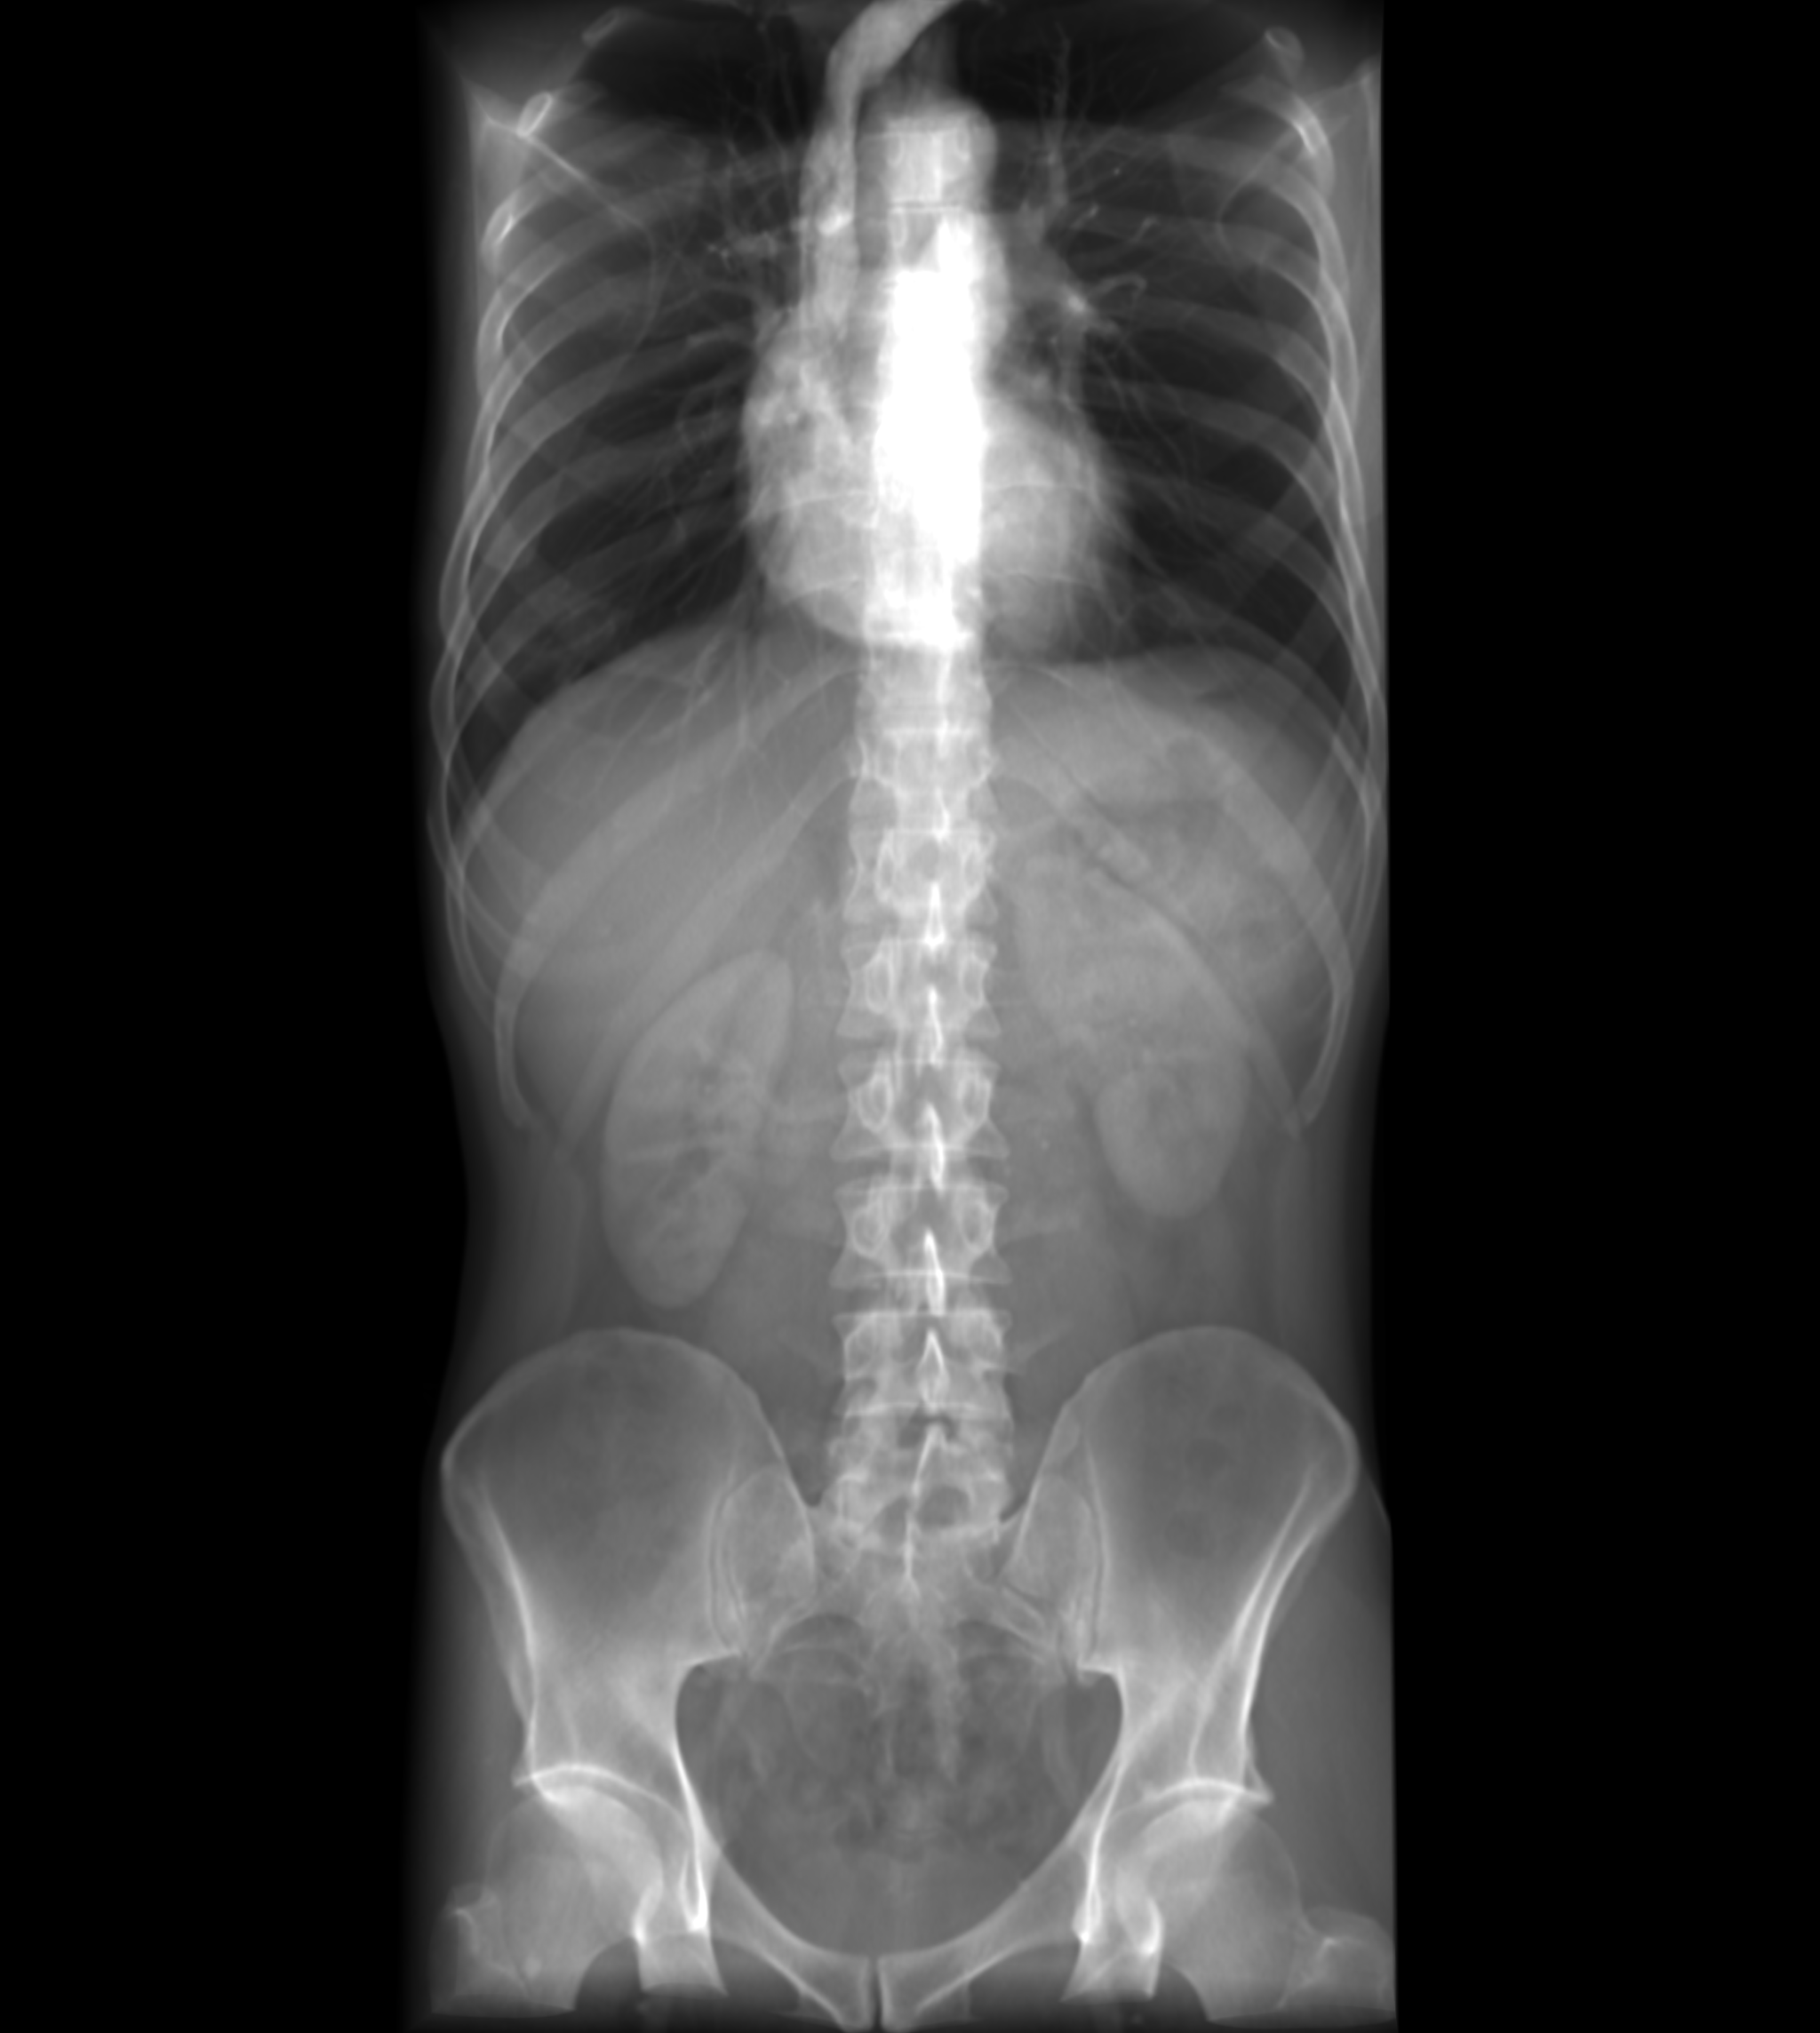
\includegraphics[width=\columnwidth]{TorsoBlendingAdditive.png}
\end{subfigure} 
\begin{subfigure}{.6\columnwidth}
    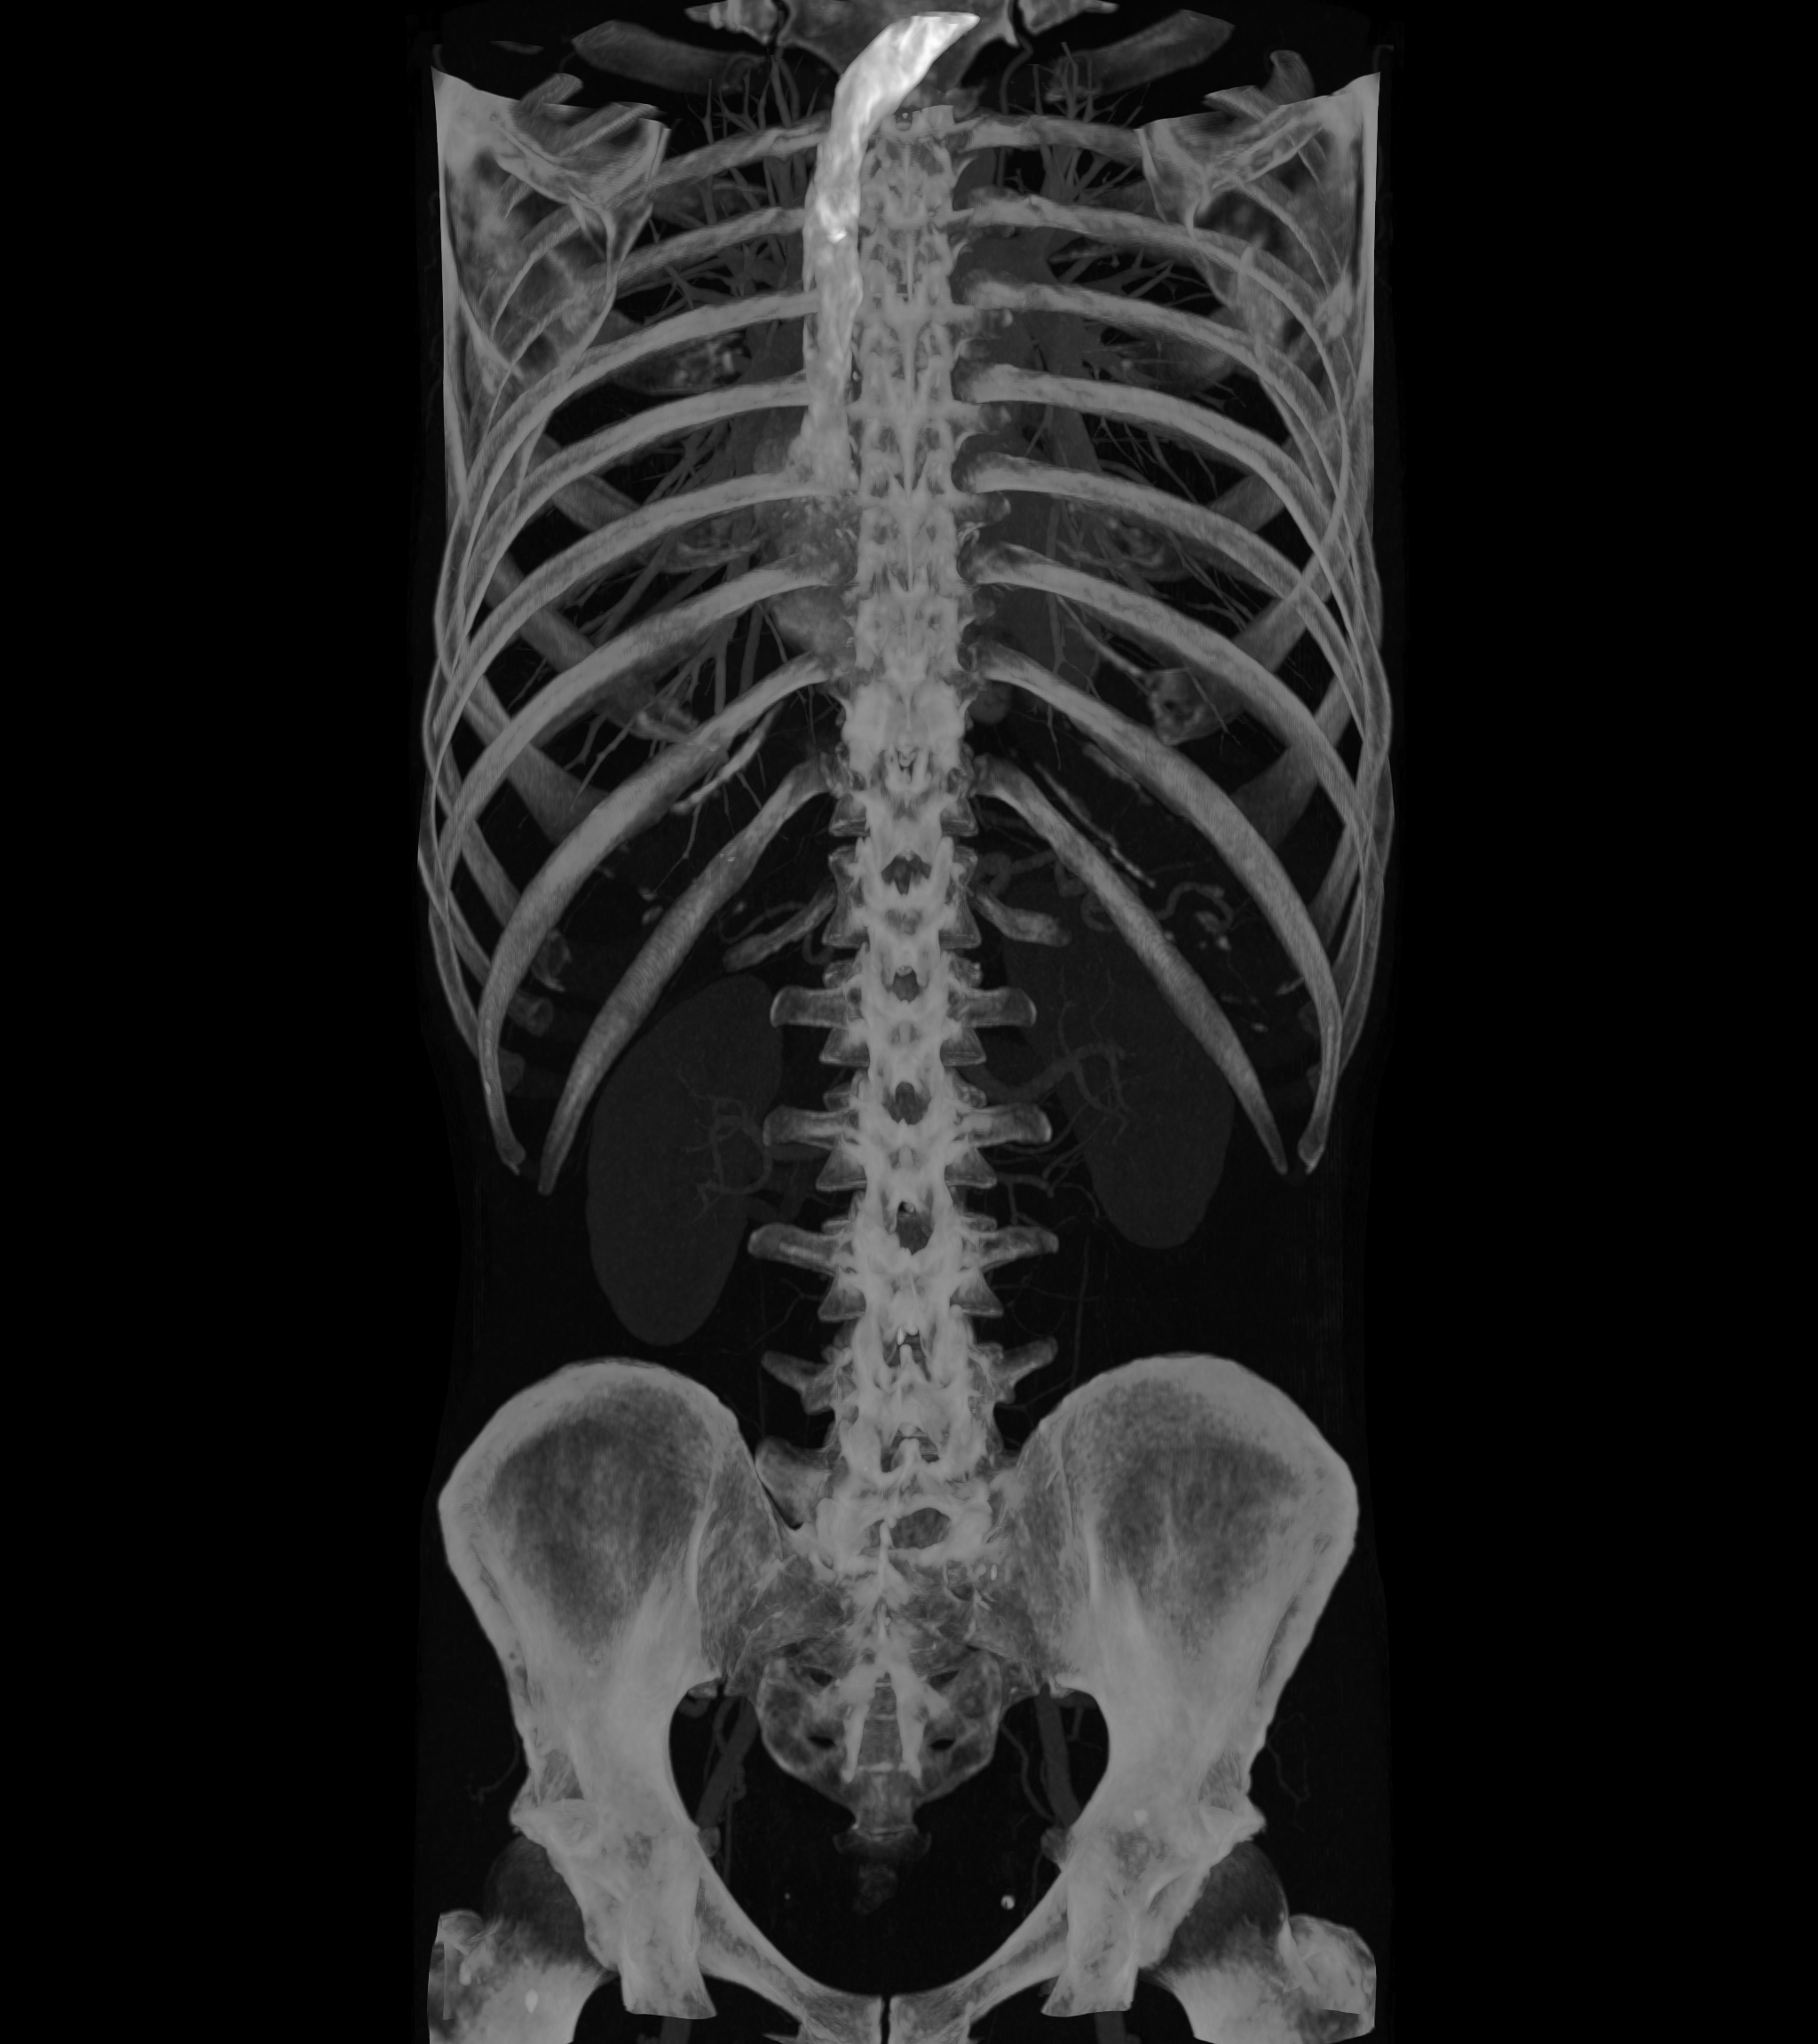
\includegraphics[width=\columnwidth]{TorsoBlendingMIP.png}
\end{subfigure}
\caption{Rendering with and without gradient opacity transfer function.}
\label{fig:blendingmodes}
\end{figure*}

\subsubsection{Masking}
Both binary and label masks are supported. With binary masks, the value in the masking volume indicates visibility of the voxel in the data volume. When a label map is in use, the value in the label map is used to select different rendering parameters for that sample.  See Figure 5 for an example of label data masks.

\subsubsection{Opacity Modulated by Gradient Magnitude}
A transfer function mapping the magnitude of the gradient to an opacity modulation value can be used to essentially perform edge detection (de-emphasize homogenous regions) during rendering. See ~\ref{fig:gradient} for an example of rendering with and without the use of a gradient opacity transfer function.

\begin{figure*}
\centering
   \begin{subfigure}[b]{0.5\textwidth}
   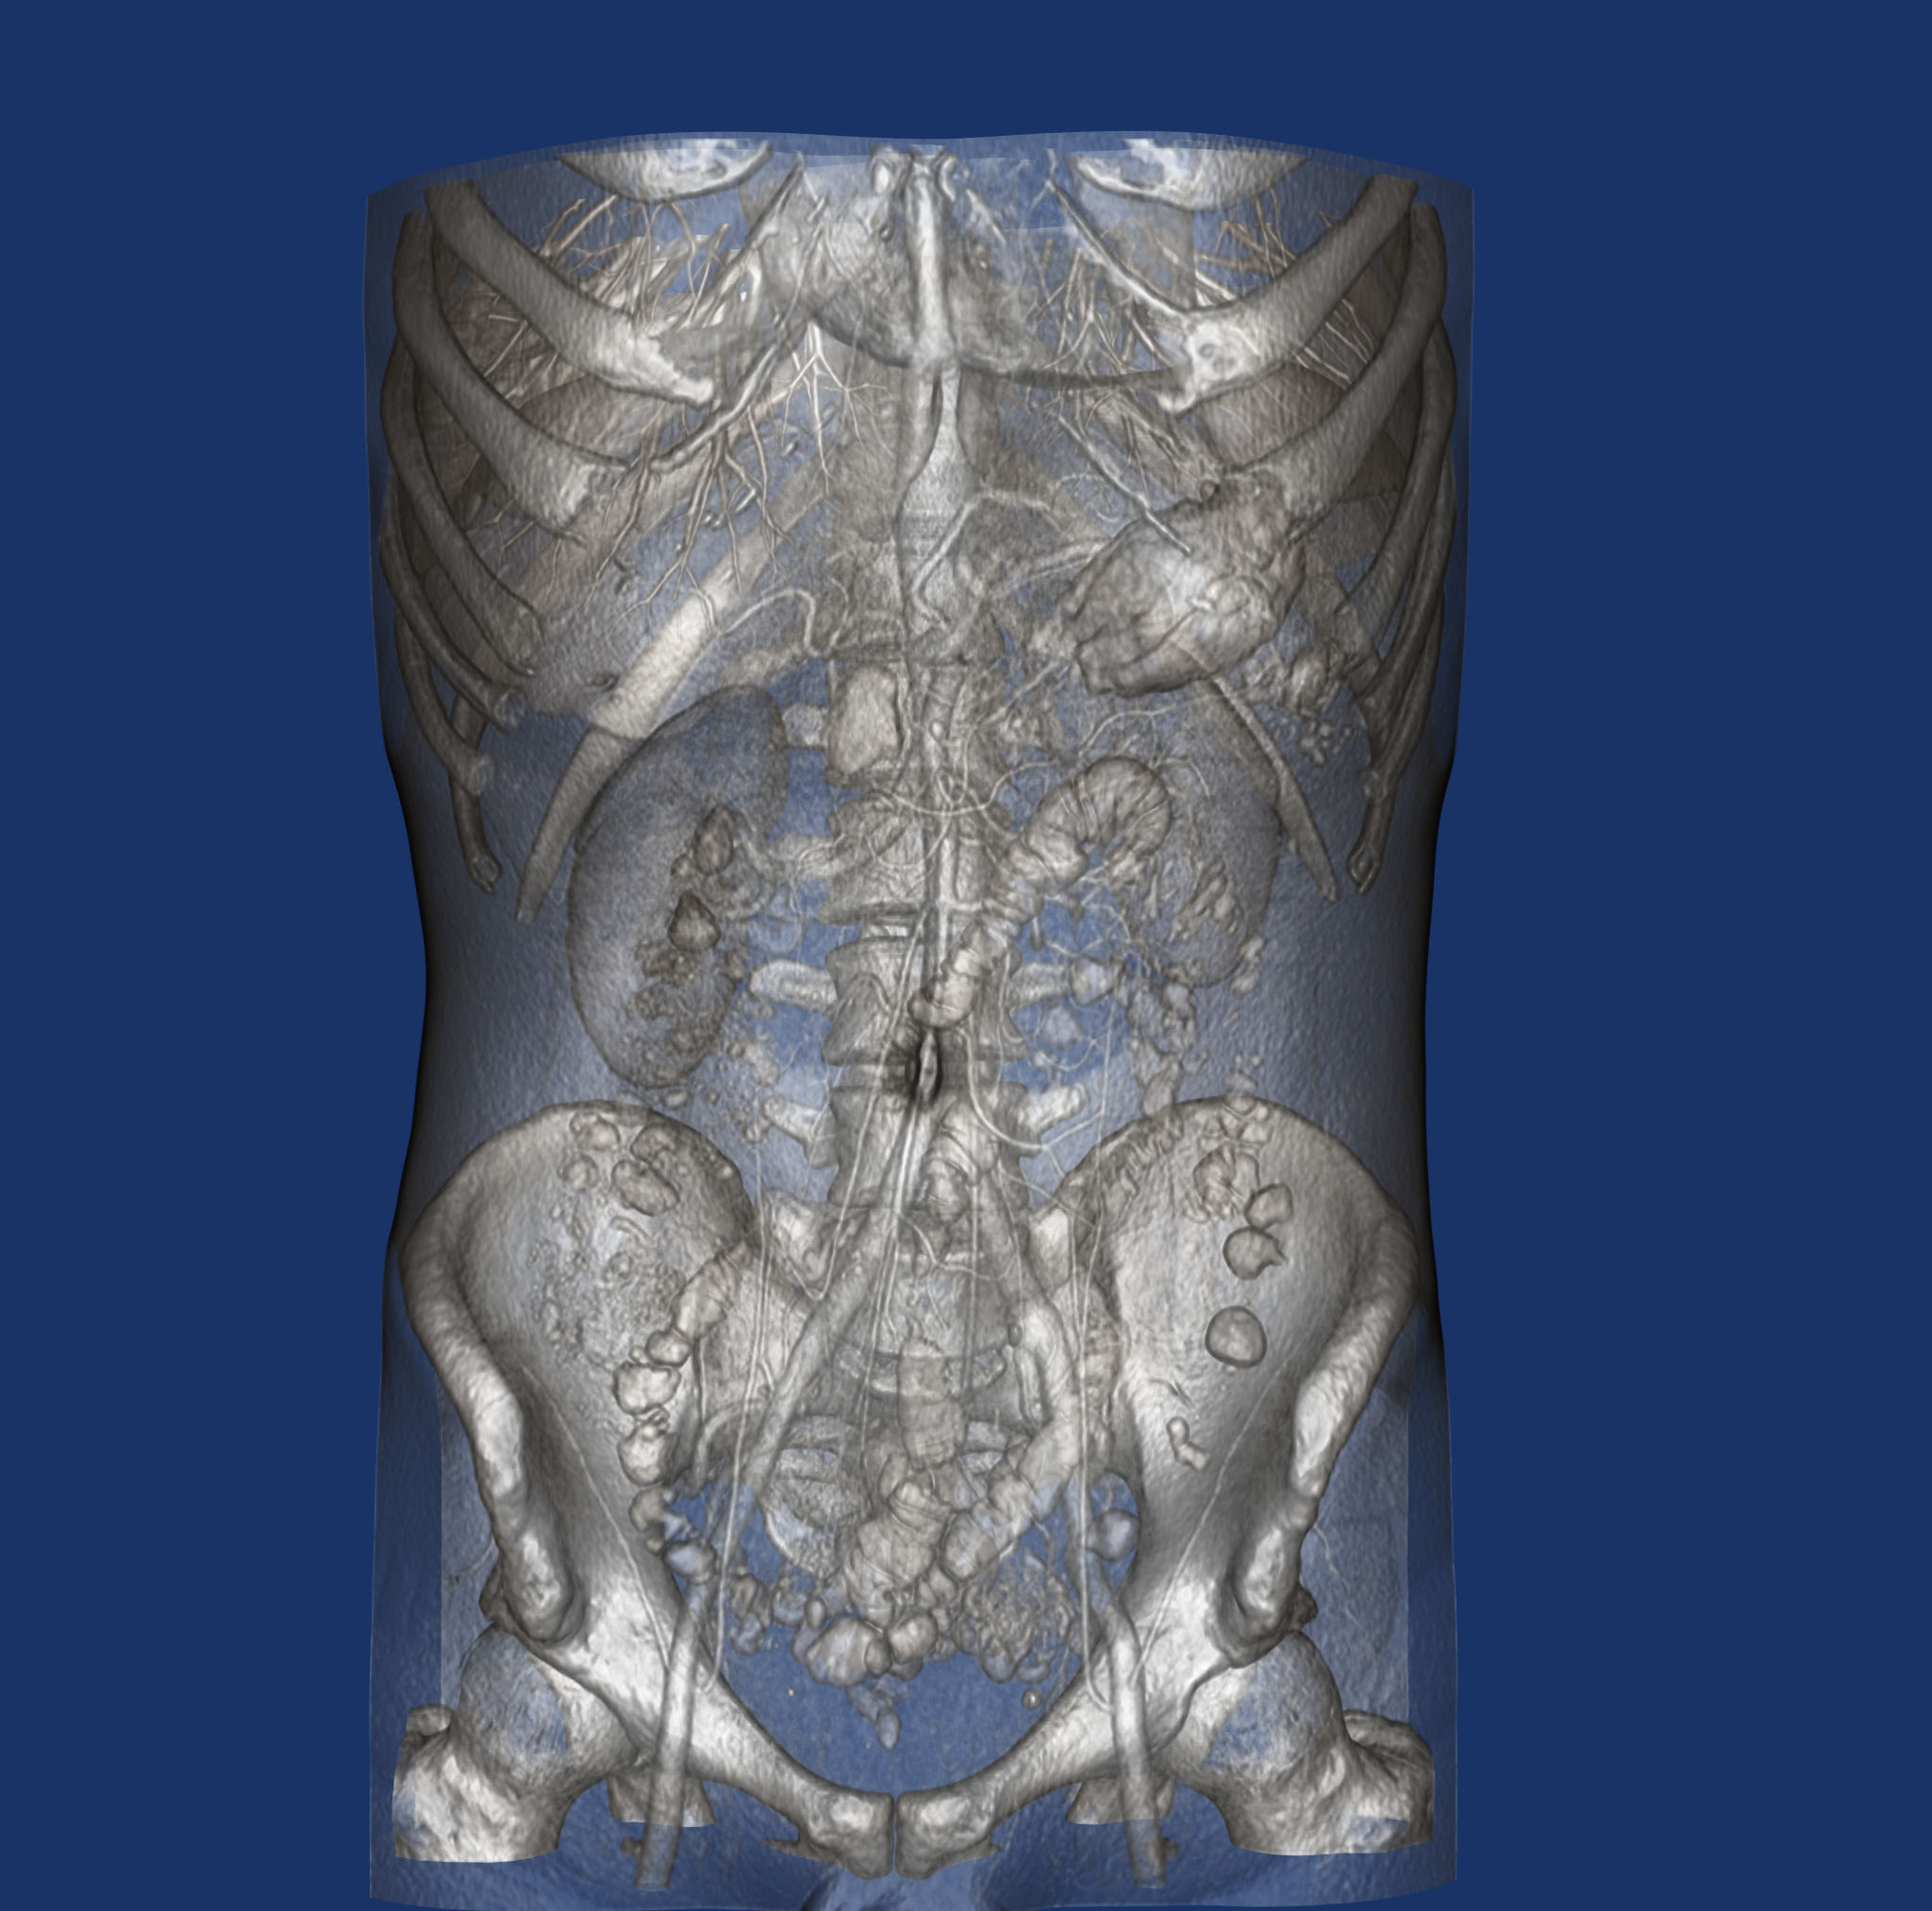
\includegraphics[width=1\linewidth]{TorsoGradient.png}
   \caption{}
   \label{fig:Ng1} 
\end{subfigure}

\begin{subfigure}[b]{0.5\textwidth}
   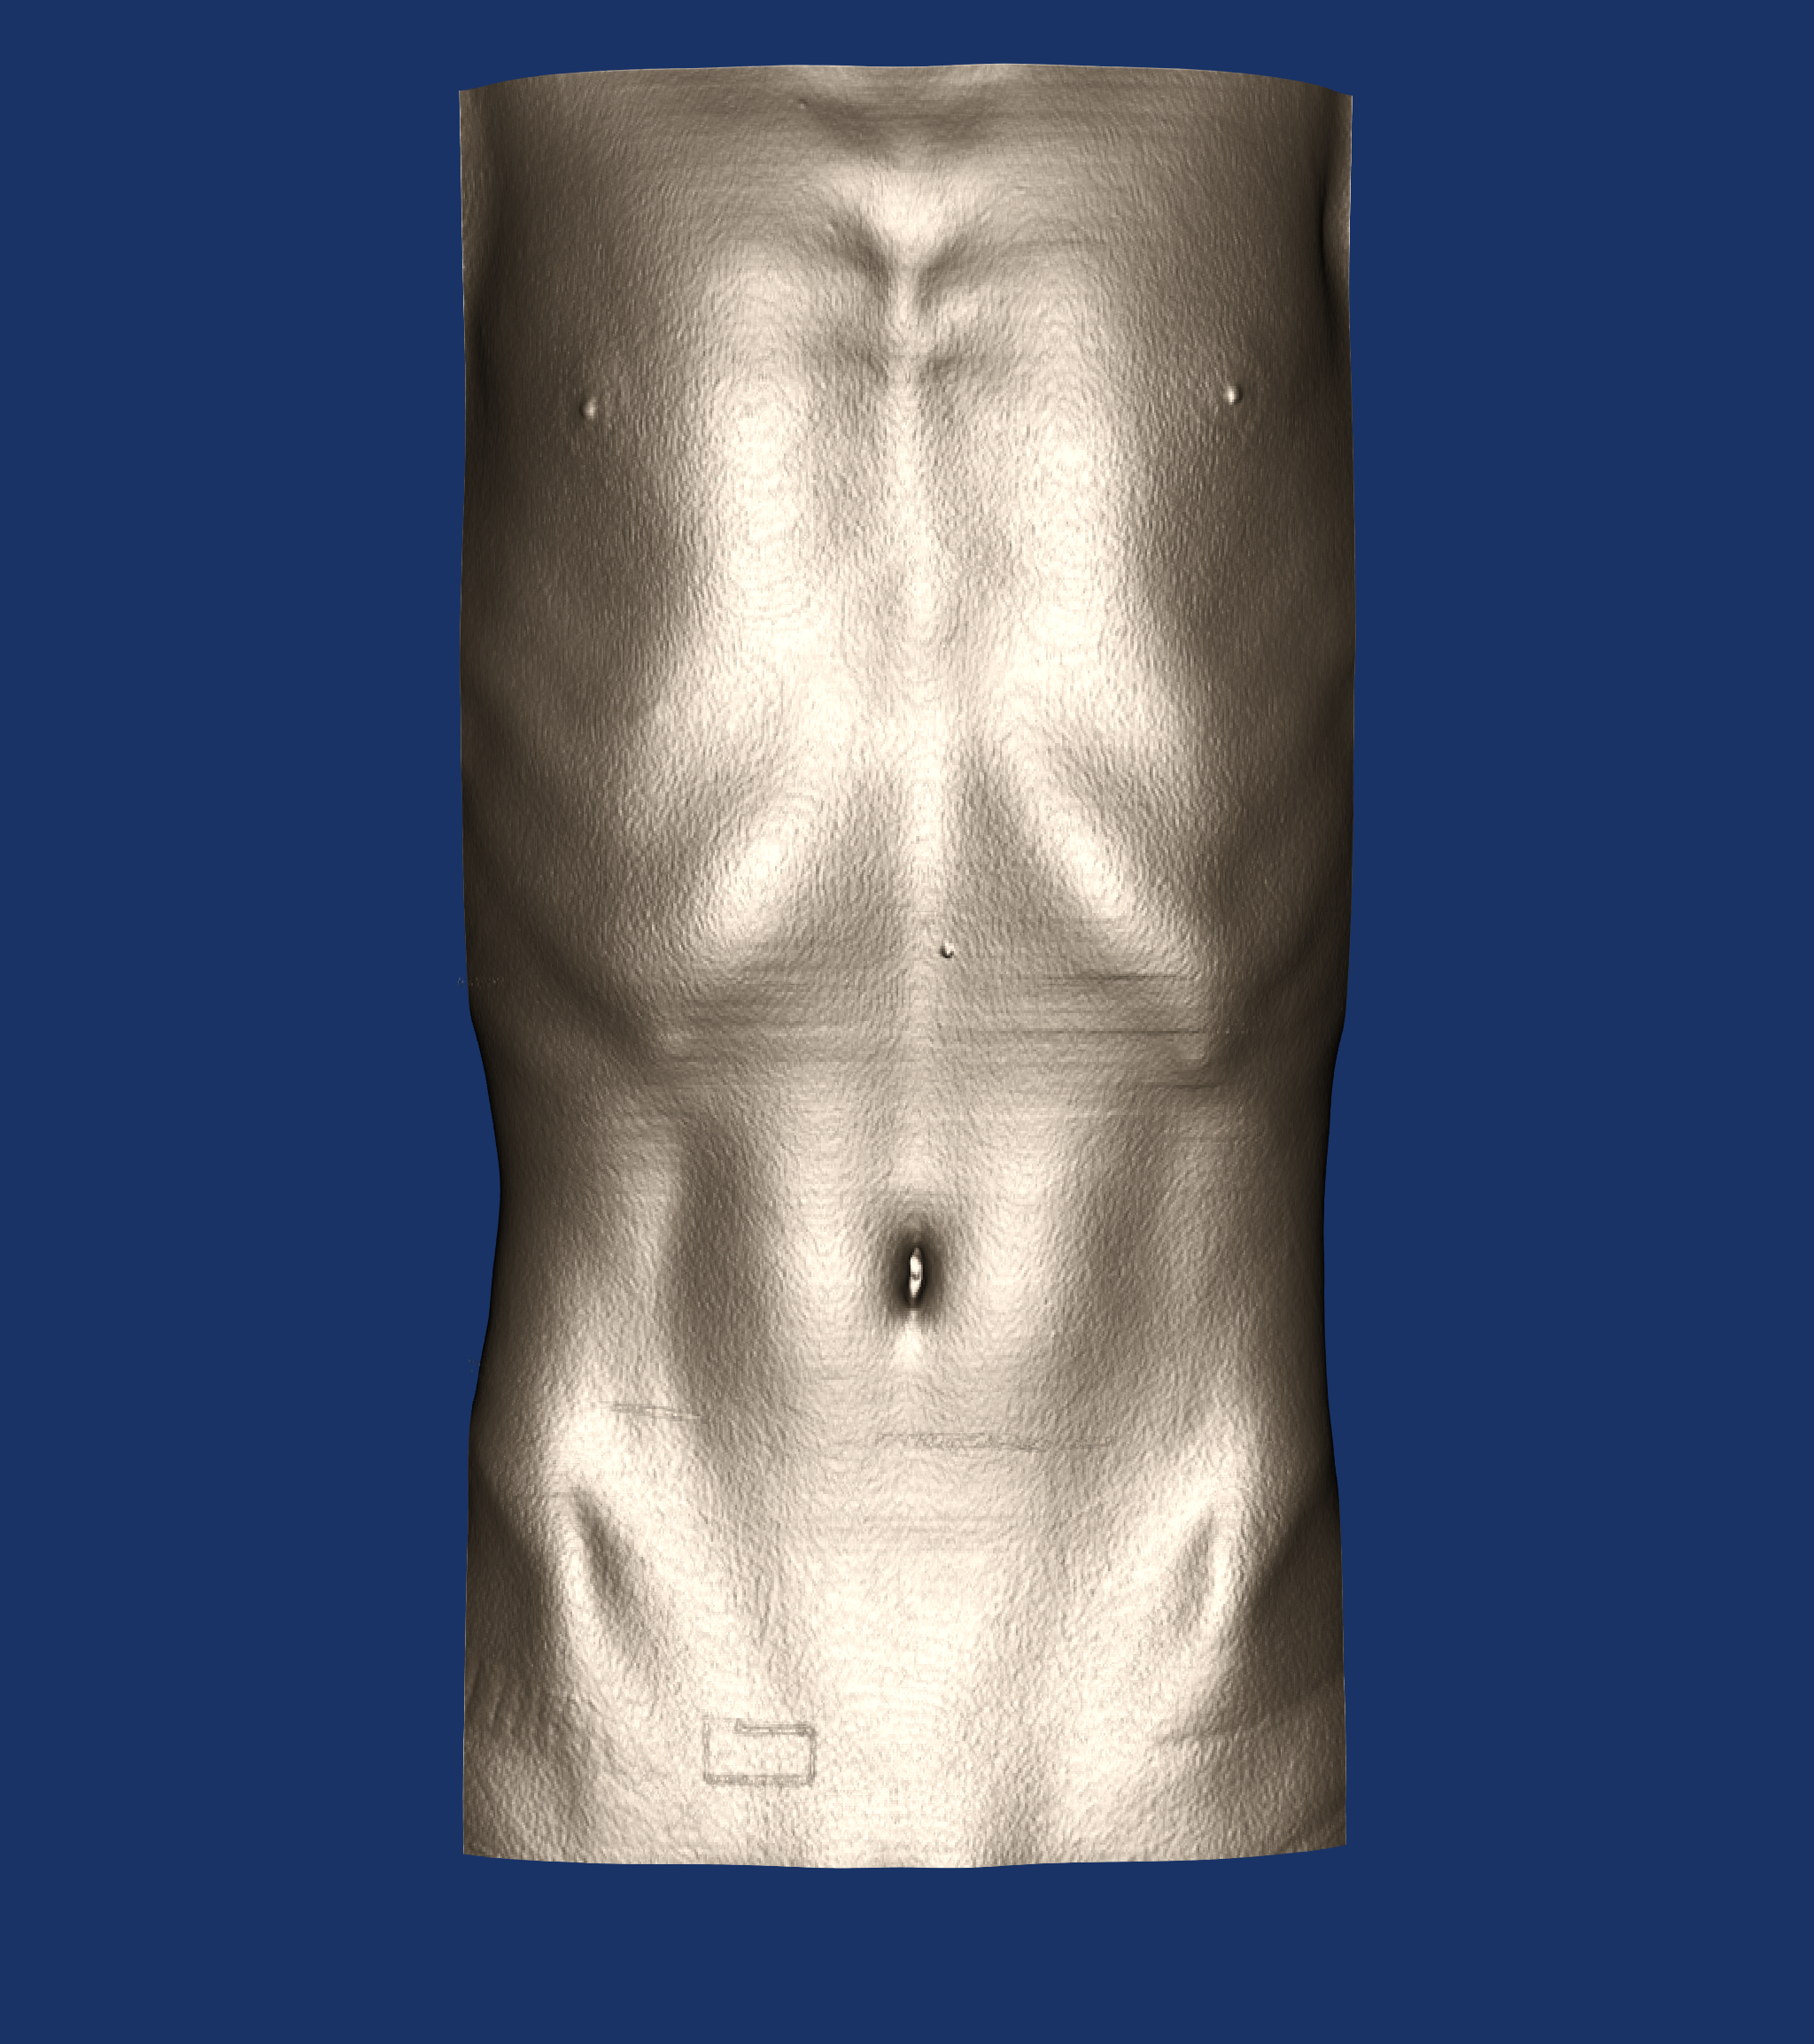
\includegraphics[width=1\linewidth]{TorsoNoGradient.png}
   \caption{}
   \label{fig:Ng2}
\end{subfigure}

\caption{Rendering with and without gradient opacity transfer function.}
\label{fig:gradient}
\end{figure*}
\section{Future Work}
\label{future-work}
At this point, we have a replacement class for vtkGPURayCastMapper that is more
widely supported, faster, more easily extensible, and supports majority of the
features of the old class. In the near future, our goal is to ensure that this
mapper works as promised by integrating it into existing VTK applications such
as ParaView and Slicer. Once these tasks are complete, we have some ideas on new
features we would like to add to this mapper (outlined below).

\subsection{2D Transfer Functions}
\label{2d-transfer-functions}
Currently, volume rendering in VTK uses three independent 1D transfer functions
to map scalar value to color, scalar value to opacity and gradient magnitude to
opacity. Increasing the number of parameters in a transfer function can improve
discrimination between structures in the volume data given that the combined
parametric information allows to disambiguate areas that fall within a given range
of those parameters simultaneously. Enhanced structure discrimination is beneficial
in medical image visualization where distinct tissues are approximately constant
in value and values transition smoothly from one tissue to the next. There is on-going
work to support 2D transfer functions combining scalar value and gradient magnitude
(the scalar field variable and its first derivative) under the the DOE Office of
Science contract DE-SC0011385 grant.

\subsection{Overlapping Volumes}
\label{overlapping-volumes}
It is currently possible to render overlapping volumes by taking advantage of
the up to 4 independent components supported by the mapper (each component
representing a different volume).
The limitation with this approach is that each of the overlapping volumes are
required to be sampled in the same grid, hence all of the volumes are required
to share the same dimensions.  Nonetheless, in order to extend the mapper to
support overlapping volumes sampled in grids with different dimensions, rays
should be casted through proxy geometry bounding the N overlapping volumes to be
rendered and separately sampling and compositing their fetched texture values in
the fragment shader.

\subsection{Improved Rendering of Labeled Data}
\label{improved-rendering-of-labeled-data}
Currently, VTK supports binary masks and only a couple of very specific versions
of label mapping. We know that our community needs more extensive label mapping
functionality – especially for medical datasets. Labeled data requires careful
attention to the interpolation method used for various parameters. (You may wish
to use linear interpolation for the scalar value to look up opacity, but,
perhaps, select the nearest label to look up the color.) We
plan to solicit feedback from the VTK community to understand the sources of
labeled data and the application requirements for visualization of this data. We
then hope to implement more comprehensive labeled data volume rendering for both
the CPU and GPU mappers.

\section{Acknowledgements}
\label{acknowledgements}
We would like to recognize the National Institutes of Health for sponsoring this
work under the grant NIH R01EB014955 - ``Accelerating Community-Driven Medical
Innovation with VTK.'' 

We thank the maintainers of the OsiriX DICOM Image
Library~\citep{osirix_osirix_2017} for providing the head (used
in~\Autoref{fig:clipping}) and torso (used in~\Autoref{fig:rendertotexture,
fig:blendingmodes, fig:gradient}) datasets used in this publication. The
Supernova (used for ~\Autoref{fig:supernova}) and Turbulent-Combustion (used
for~\Autoref{fig:paraview-turbulent-combustion}) datasets were obtained from
VisFiles~\citep{visfiles_visfiles_2007}. The supernova dataset is made available
by John Blondin at the North Carolina State University through US Department
of Energy's SciDAC Institute for Ultrascale Visualization.The turbulent
combustion dataset is made available by Jackqueline Chen at Sandia
Laboratories through US Department of Energy's SciDAC Institute for Ultrascale
Visualization. We would also like to thank Jianwei (John) Miao from University
of California at Los Angeles and Robert Hovden from Cornell University for
granting us permission to use the~\ce{PtCu} (used in~\Autoref{fig:ptcu-grad})
and~\ce{Co2P} (used in~\Autoref{fig:tomviz-cop}) nanoparticle datasets. The
cactus sample dataset (used in~\Autoref{fig:jittering}) is courtesy of Michael
Holland and Dula Parkinson from Advanced Light Source, Lawrence Berkeley National
Laboratory.


\bibliographystyle{abbrv}
\bibliography{VTKVR}
\end{document}





